\chapter{Umsetzung und Evaluation des optimierten Prozesses}

%-> Konkrete Umsetzung/ Ausgestaltung des optimierten Prozesses im System 

%-> Generelles Ziel SAP-Consulting: Immer Standard, wenn irgendwie möglich

\section{Lösung 1: Anpassung des Standards} \label{sec:Kapitel41}

\subsubsection{Grundlegendes}

Im Folgenden soll die Umsetzung des Soll-Konzepts durch eine Anpassung des SAP-Standards vorgestellt werden. Des geschieht konkret durch ein Customizing der Fiori-App ''Massenänderungen an zentralen Einkaufskontrakten''. SAP Fiori ist ein Framework für die Entwicklung und Bereitstellung von SAP-Apps. Durch ein einheitliches und rollenbasiertes Layout entsteht eine intuitiv bedienbare und konsistente Benutzeroberfläche. Da Fiori Apps responsive sind, können diese auf verschiedenen Endgeräten genutzt werden, um die Produktivität der Nutzer zu steigern. Insgesamt soll Fiori die UX von SAP-Anwendungen, vor allem für unerfahrenere Nutzer, verbessern.\footcite[Vgl.][]{praxis_sap_fiori_allgemein_2024}

\subsubsection{Aufbau der App}

\begin{figure}[H]
    \centering
    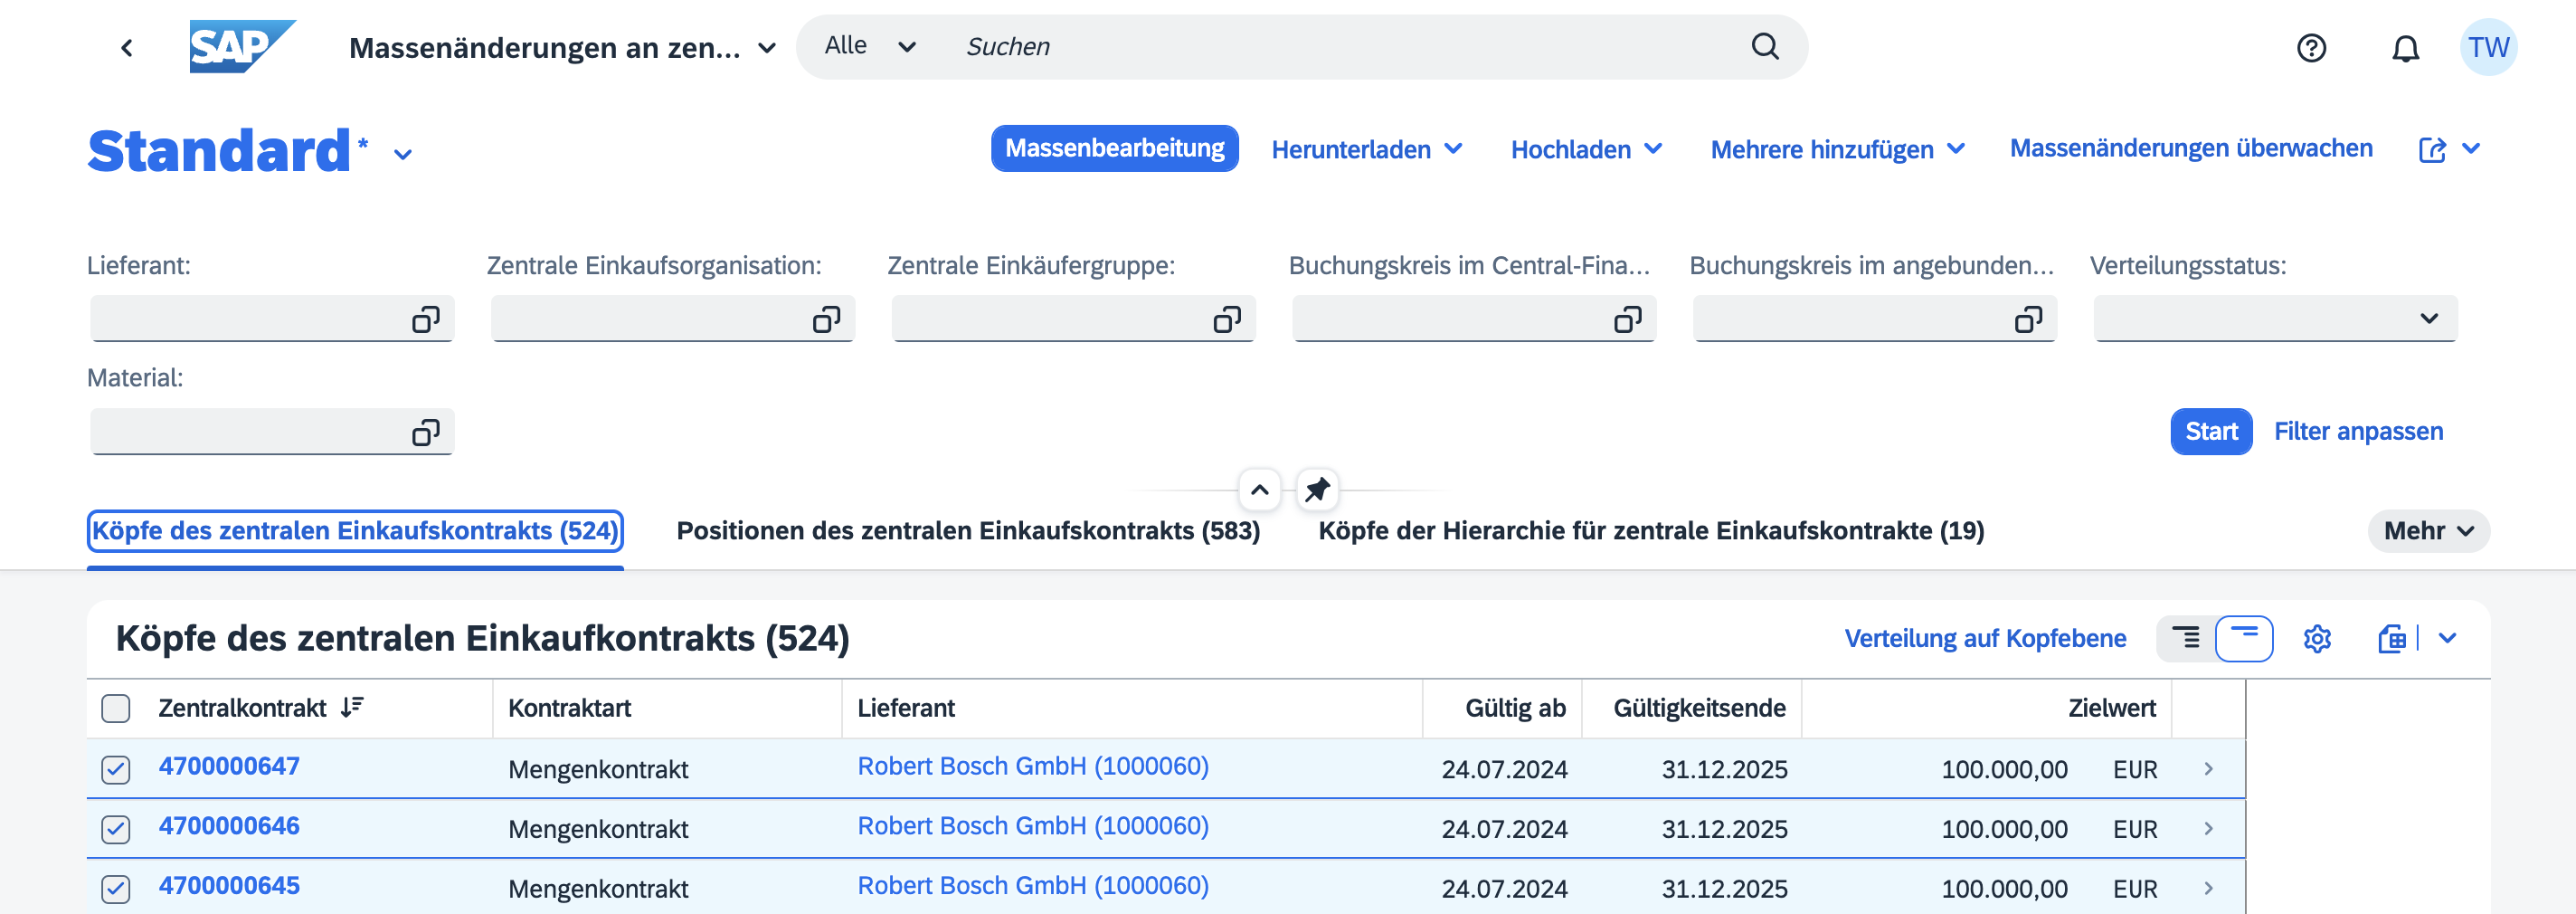
\includegraphics[height=5.31cm]{Bilder/Praxisteil-S-Schritt-1.png}
    \caption[Standard Customizing, Massenbearbeitung Central Contracts, Auswahl der Zentralkontrakte]{Standard Customizing, Massenbearbeitung Central Contracts, Auswahl der Zentralkontrakte. Eigene Darstellung}
    \label{fig:PraxisSSchritt1}
\end{figure}

Zuerst wird der allgemeine Prozessfluss und Aufbau der App beschrieben. Einschränkend ist zu nennen, dass die Fiori-App selbst, aufgrund von Einschränkungen der Software durch SAP, nicht anpassbar ist. Deshalb müssen die folgenden Ausführungen als gegeben angenommen werden. Dies hat zur Folge, dass das Konzept im Bezug auf die Prozessstruktur nicht exakt umgesetzt werden kann. Abbildung \ref{fig:PraxisSSchritt1} zeigt den Einstiegspunkt eines Benutzers nach dem Öffnen der App. Im oberen Bereich der Seite befindet sich die allgemeine Fiori Navigation, über die man auf die Übersichtsseite aller Fiori Apps gelangen oder nach anderen Apps suchen kann. Zudem befinden sich rechts oben das Benutzerprofil und Benachrichtigungen. Darunter können die Ansicht der App ausgewählt und verschiedene Aktionen ausgeführt werden. Der Button ''Massenbearbeitung'' führt die Online-Massenänderungsmodus aus. Dieser bietet die Möglichkeit ein oder mehrere Felder in allen ausgewählten Verträgen mit einem Wert zu überschreiben. Da dies nicht das Ziel des Konzepts ist, wird diese Funktion im Folgenden au\ss er Acht gelassen. Konkret wird die Offline-Massenänderung betrachtet: Hier können über die Knöpfe ''Herunterladen'' und ''Hochladen'' eine Excel-Datei herunter- und wieder hochgeladen werden. Nachdem die Datei mit den jeweiligen Ist-Daten heruntergeladen wurde, können innerhalb der Systemgrenzen beliebige Änderungen vorgenommen werden. Beispielsweise können für verschiedene Verträge/ Vertragspositionen jeweils anders geändert werden. Zudem können auch komplette Zentralkontrakte hinzugefügt oder gelöscht werden. Nachdem alle Änderungen voregenommen wurden, wird die Excel-Liste wieder ins System hochgeladen. An diesem Punkt kann sich der Einkäufer entscheiden, ob die Änderungen direkt übernommen, oder zuerst eine Simulation durchgeführt werden soll.\footcite[Vgl.][]{theorie_sap_fiori_make_mass_changes_2024} Über den Button ''Massenänderungen überwachen'' öffnet sich die gleichnamige App und der Benutzer kann in beiden Fällen das Ergebnis mit eventuellen Warnungen und Fehlermeldungen einsehen. Im Falle der Simulation kann diese hier final im System übernommen oder verworfen werden.\footcite[Vgl.][]{theorie_sap_fiori_monitor_mass_changes_2024} Die Funktion ''Weitere hinzufügen'' ermöglicht es, Verteilungsschlüssel festzulegen, die bestimmen, welche Mengen welcher Teile in den gewählten Verträgen für welche Werke bestimmt sind. Letztere ist ebenfalls im Anwendungskontext nicht relevant. Unter den eben genannten Knöpfen befinden sich Filtermöglichkeiten, um die Anzeige der Verträge zu verfeinern. Im Auswahlbereich der App stehen dem Facheinkäufer drei Bereiche zur Verfügung: Köpfe und Positionen zentraler Einkaufskontrakte, sowie dieselben Möglichkeiten der Hierarchie der zentralen Einkaufskontrakte. Da die letztere Möglichkeit von BMW nicht eingesetzt wird, wird diese nachfolgend nicht betrachtet. Allgmein lässt sich aber sagen, dass Massenänderungen auf Vertragsebene oder auf Positionsebene vorgenommen werden können. Der Endanwender kann nun die gewünschten Verträge, sowie zugehörigen Positionen, die er bearbeiten möchte selektieren. Im Kundenkontext ist dies trivial, da jeder Vertrag nur eine Position enthält. Diese werden in einer Tabelle aufgelistet. In Abbildung \ref{fig:PraxisSSchritt1} werden in den Spalten noch die Attribute des Standards angezeigt, diese können jedoch analog zu den in \ref{sec:Kapitel422} gewählten Attributen angepasst werden.

\subsubsection{Massenbearbeitung in Excel}

Nachdem der Einkäufer die gewünschten Zentralkontrakte inklusive Positionen selektiert hat, können deren Daten als Excel Datei angepasst werden. In diesem Bereich ist die SAP-Lösung flexibel konfigurierbar. So können benutzerdefiniert mehrere Arbeitsblätter angelegt und diese fast beliebig mit Feldern des Central Contracts befüllt werden. Im Folgenden soll diese Excel-Datei vorgestellt werden. Jede zu bearbeitende Kategorie wird durch ein Tabellenblatt dargestellt.

\begin{figure}[H]
    \centering
    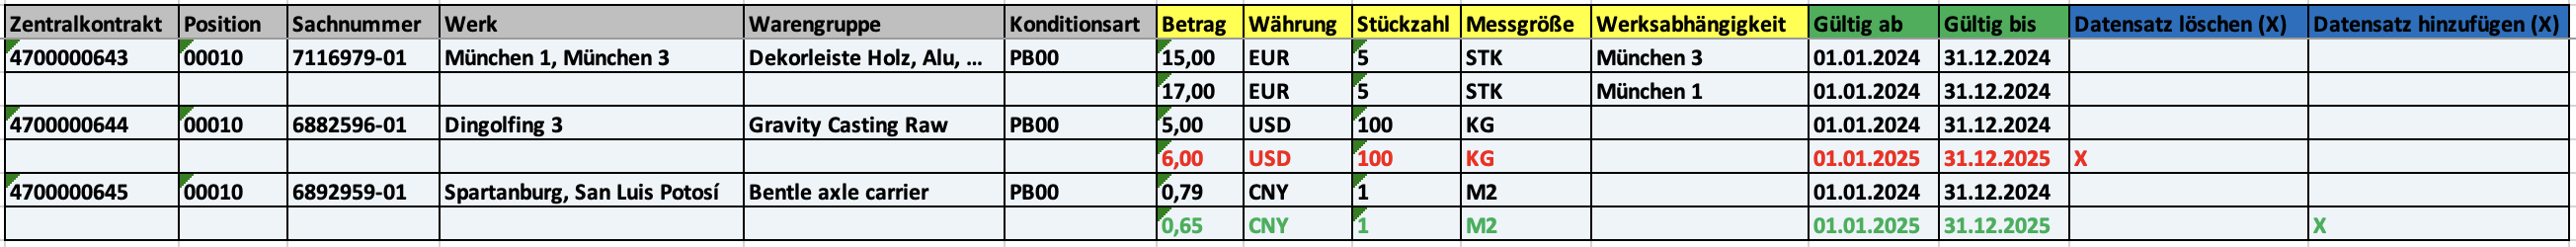
\includegraphics[height=1.03cm]{Bilder/Praxisteil-S-Schritt-2.png}
    \caption[Standard Customizing, Massenbearbeitung Central Contracts, Bearbeitung des Basispreises]{Standard Customizing, Massenbearbeitung Central Contracts, Auswahl der Zentralkontrakte. Eigene Darstellung}
    \label{fig:PraxisSSchritt2}
\end{figure}

Abbildung \ref{fig:PraxisSSchritt2} stellt die Bearbeitung des Basispreises im ersten Schritt dar. Allgemein sind Spalten, deren Spaltenköpfe grau markiert sind lediglich informativ, um dem Einkäufer die Identifikation der gewählten Verträge zu erleichtern. Spalten mit gelben Spaltenköpfen enthalten fachliche Daten des Zentralkontrakts, die editiert werden dürfen. Grün hinterlegte Spaltenköpfe enthalten die zeitlichen Gültigkeiten einzelner Konditionen/ Rohstoffe. Diese können aufgrund von Limitationen der Software nicht in einen Vorauswahlschritt extrahiert werden. Die blauen Spalten sind lediglich technischer Natur, falls ein Facheinkäufer einen Datensatz hinzufügen oder löschen möchte. In diesem Fall müsste eine der beiden Spalten mit ''X'' markiert werden. Sollte ein Datensatz so gelöscht werden, wird jedoch nur \zB die jeweilige Kondition/ Rohstoff gelöscht, nicht die gesamte Vertragsposition oder der gesamte Vertrag. Wenn beispielsweise eine neue Kondition hinzugefügt werden soll, muss eine Spalte kopiert, die jeweiligen Daten ausgetauscht und die Spalte ''Datensatz hinzufügen'' markiert werden.

\section{Lösung 2: Entwicklung einer kundenspezifischen Lösung}

Die zweite Möglichkeit die Kundenanforderungen umzusetzen ist die Entwicklung einer kundenspezifischen Lösung. Allgemein bietet sich im konkreten Fall die Entwicklung einer kundeneigenen Fiori-App an, über die die Daten im System gepflegt werden können. Fiori bietet mehrere Vorlagen an, die als Basis für die Entwicklung einer App genutzt werden können. Für den betrachteten Prozess bietet sich die Vorlage ''Wizard-Floorplan'' an, da diese eine schrittweise Benutzerführung durch mehrstufige Prozesse bietet. So können komplexe Aufgaben in kleinere Schritte unterteilt werden zwischen denen der Benutzer navigieren kann und bei denen er bei Bedarf Hilfestellungen und Fehlermeldungen erhält. So soll die UX gesteigert und die Fehlerquote gesenkt werden \parencite[Vgl.][]{praxis_sap_wizard_floorplan_2024}. Im Folgenden soll der Aufbau dieses Floorplans anhand des ersten Prozessschrittes exemplarisch beschrieben werden.

\subsubsection{Auswahl des Zeitintervalls}

\begin{figure}[H]
    \centering
    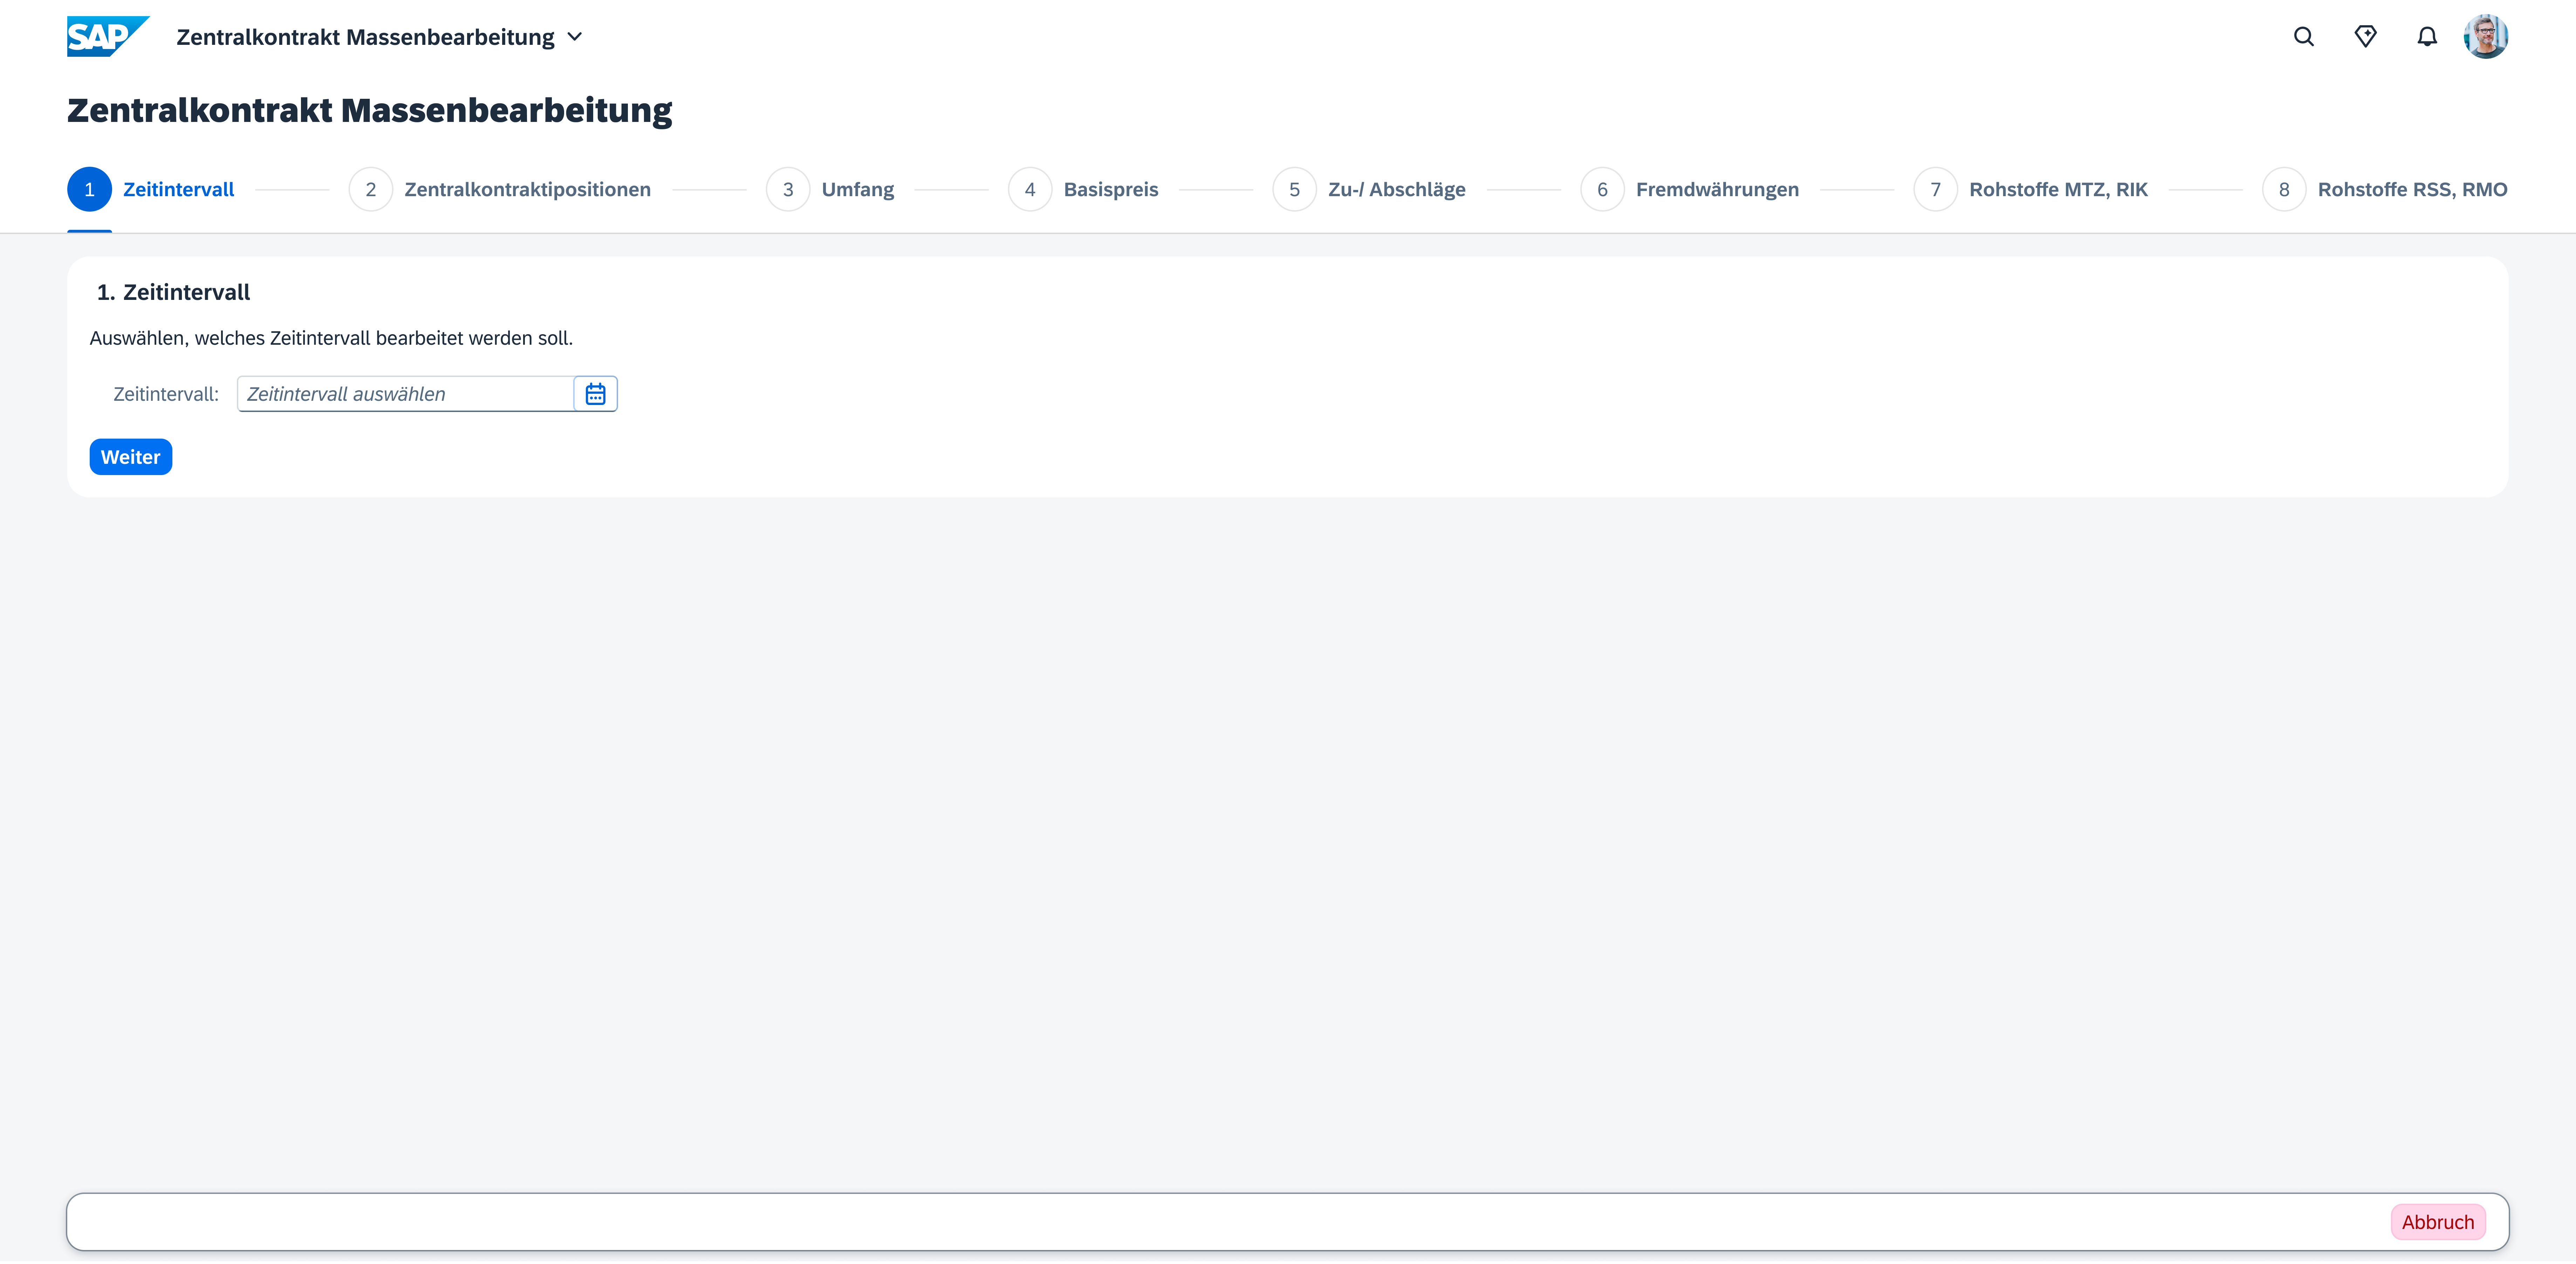
\includegraphics[height=7.37cm]{Bilder/Praxisteil-KL-Schritt-1.png}
    \caption[Kundenentwicklung, Massenbearbeitung Central Contracts, Auswahl des Zeitintervalls]{Kundenentwicklung, Massenbearbeitung Central Contracts, Auswahl des Zeitintervalls. Eigene Darstellung}
    \label{fig:PraxisKLSchritt1}
\end{figure}


In Abbildung \ref{fig:PraxisKLSchritt1} ist der erste Schritt des Prozesses dargestellt. Der Header der App enthält analog zu  Kapiel \ref{sec:Kapitel41} die allgemeine Fiori Navigation. Unter dem Titel der App befindet sich eine Übersicht über die Abfolge der Prozessschritte mit einer Anzeige über den jeweiligen Fortschritt des Prozesses. Darunter beginnt der eigentliche Inhalt der App. Dieser unterscheidet sich in jeder Phase. In der Abbildung kann der Benutzer ein Zeitintervall mithilfe eines Auswahlfeldes eingeben. In diesem Zeitintervall werden alle folgenden Änderungen vorgenommen. Sollte sich das gewählte Intervall über mehrere Instanzen des Basispreises erstrecken erscheint eine Warnung, da bei Fortfahren einzelne Intervalle nicht nur verkürzt, sondern vollständig überschrieben werden. Sollte kein oder ein ungültiges Zeitintervall ausgewählt werden, erscheint eine Fehlermeldung, und der Prozess kann nicht fortgesetzt werden, bis ein gültiger Zeitraum ausgewählt wurde. Dies gilt auch für den Fall, dass, abhängig von der jeweiligen Berechtigung eines Benutzers, ein Zeitraum von mehr als zwölf bzw. 36 Monaten in der Vergangenheit gewählt wird. Nachdem der Einkäufer einen Zeitraum durch Klicken auf den Kalender ausgewählt hat, gelangt man durch den Button ''Weiter'' zum nächsten Schritt. Alternativ kann der Benutzer den Prozess durch den Knopf ''Abbruch'' abbrechen oder durch den Button ''Zurück'' einen Schritt zurückgehen.\footnote{Der Button ist auf Abbildung \ref{fig:PraxisKLSchritt1} nicht vorhanden, da es sich um den ersten Schritt handelt. In den folgenden Schritten ist dieser in der Leiste unten links zu sehen}

\subsubsection{Auswahl der Zentralkontrakte} \label{sec:Kapitel422}

\begin{figure}[H]
    \centering
    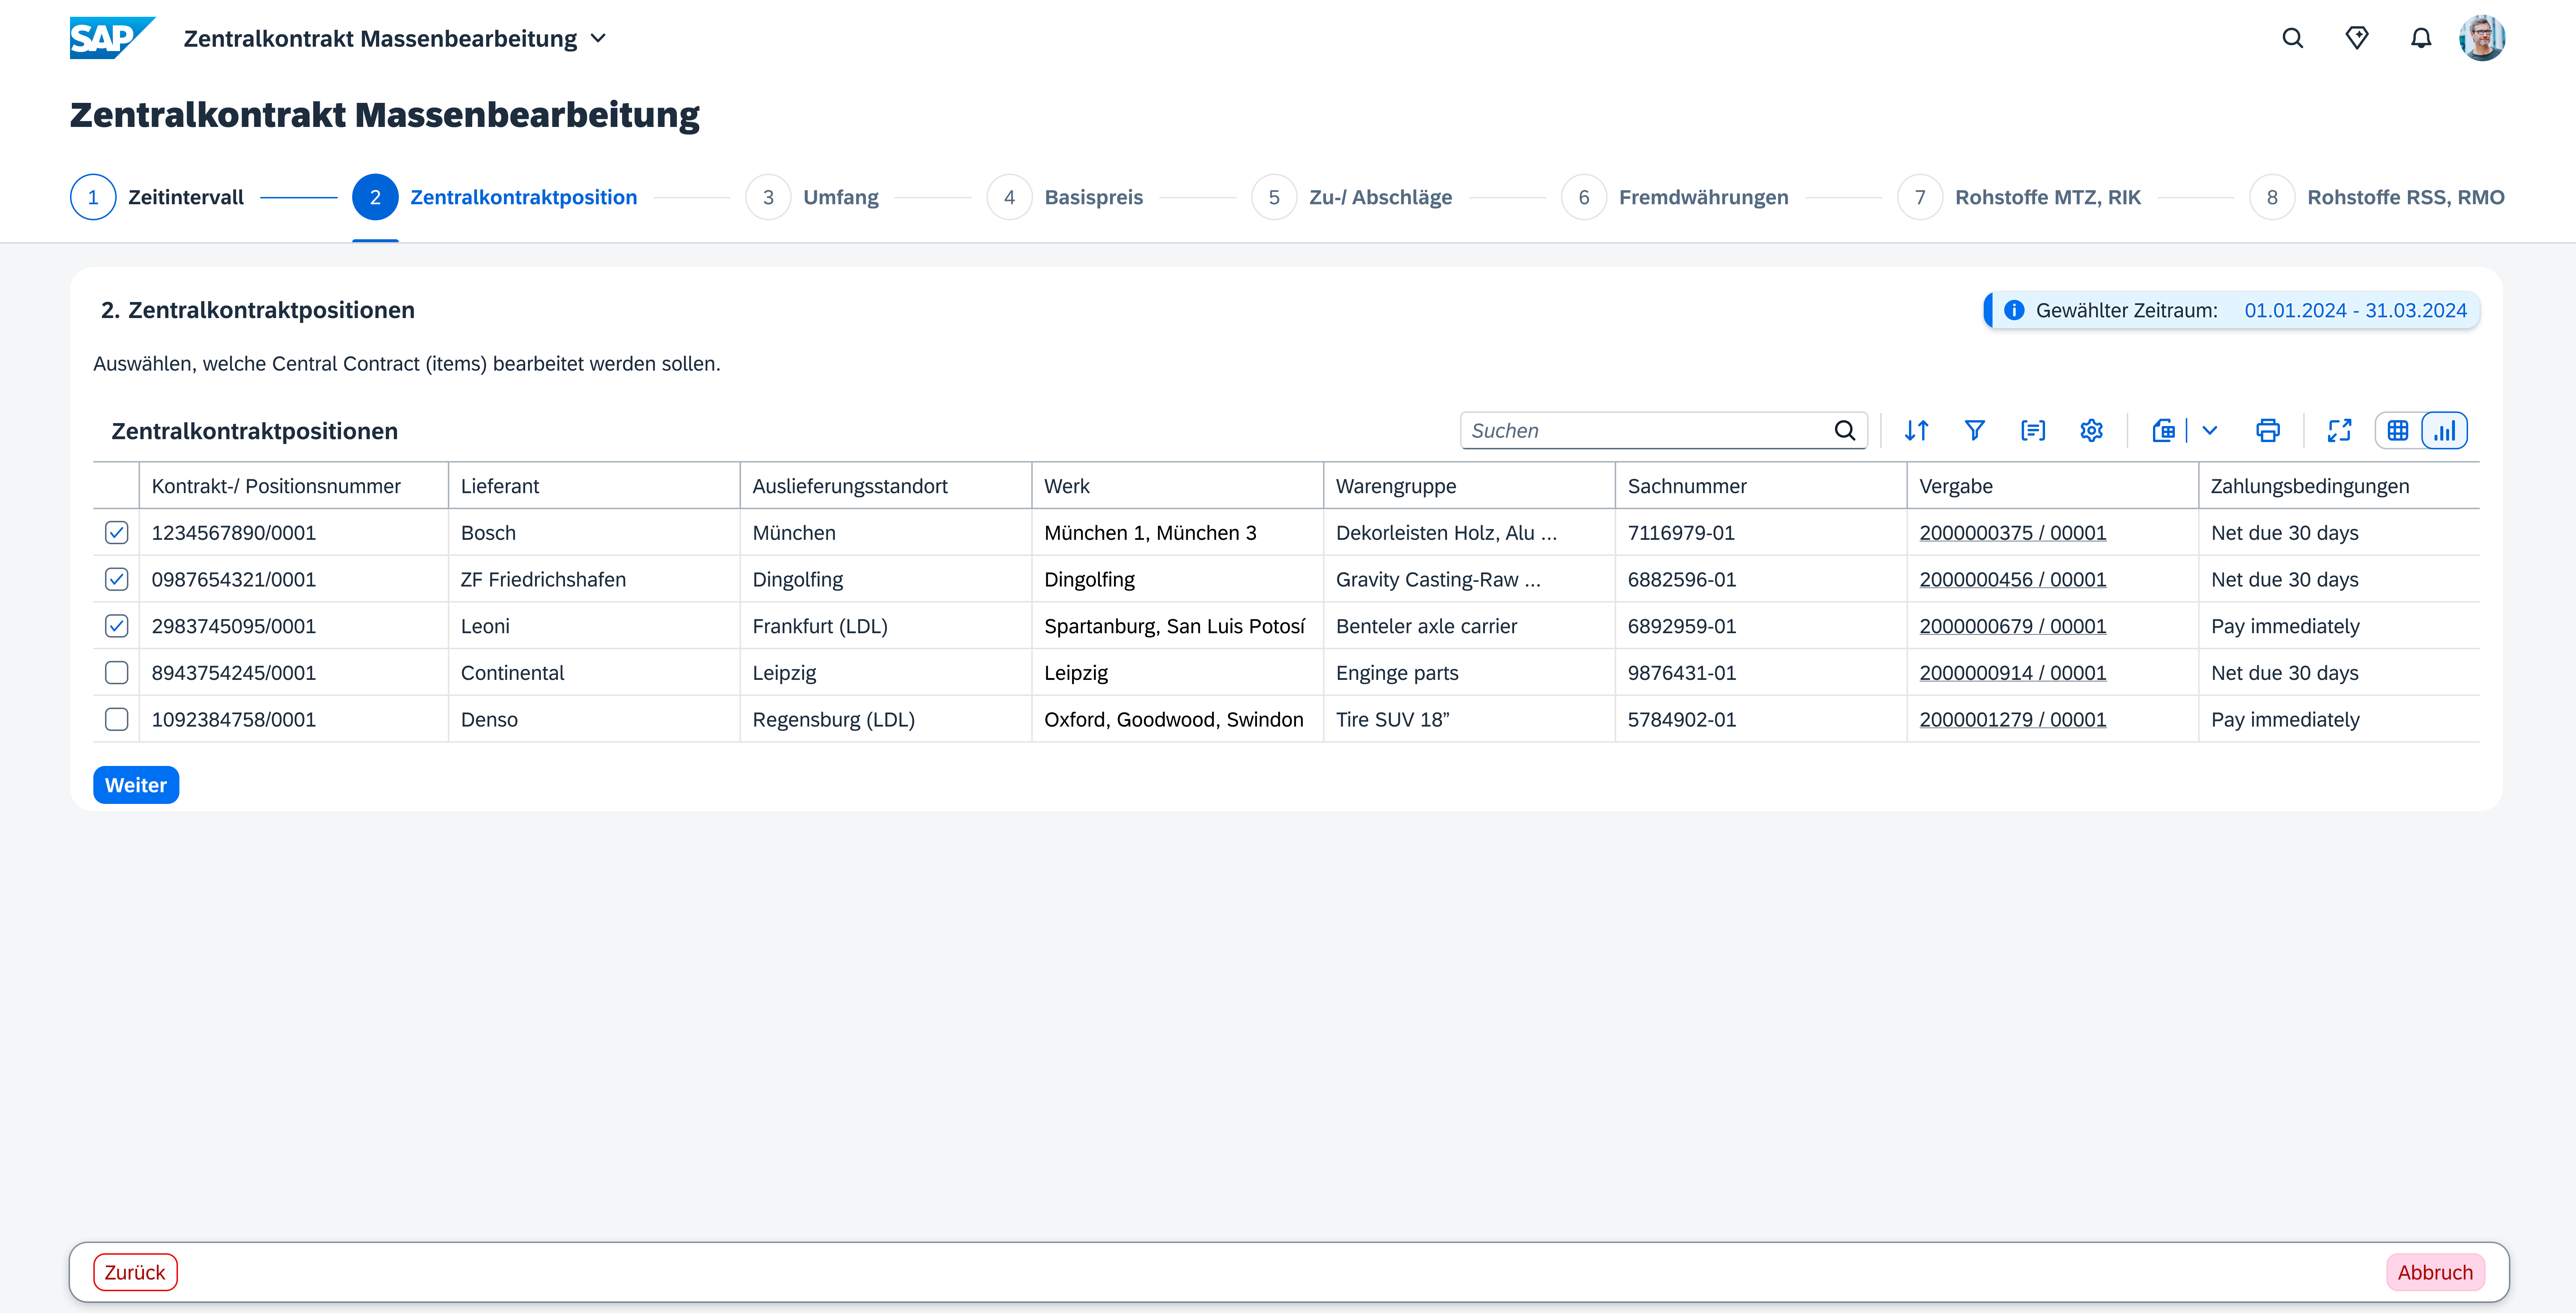
\includegraphics[height=7.66cm]{Bilder/Praxisteil-KL-Schritt-2.png}
    \caption[Kundenentwicklung, Massenbearbeitung Central Contracts, Auswahl der Zentralkontrakte]{Kundenentwicklung, Massenbearbeitung Central Contracts, Auswahl der Zentralkontrakte. Eigene Darstellung}
    \label{fig:PraxisKLSchritt2}
\end{figure}

Abbildung \ref{fig:PraxisKLSchritt2} zeigt den zweiten Schritt des Prozesses. Hier kann der Benutzer die Zentralkontrakte auswählen, die er bearbeiten möchte. Dazu stehen Filter-, Such- und Sortierfunktionen zur Verfügung. Des Weiteren kann die Tabelle exportiert und deren Darstellung verändert werden. Jedoch sind für den Facheinkäufer nur die Central Contracts sichtbar, die aufgrund der jeweiligen Rolle in dessen Verantwortungsbereich liegen. Durch Klicken auf die Checkboxen werden die Kontrakte selektiert. Zur Identifikation der zu ändernden Kontrakte wurden durch die Facheinkäufer wichtige Attribute identifiziert, die in der Tabelle abgebildet sind. Diese wird über eine Schnittstelle zum Zentralkontrakt befüllt. Auf einige Attribute soll nachfolgend genauer eingegangen werden. Die Kontrakt-/ Positionsnummer ist die eindeutige ID eines Zentralkontrakts. Deren letzter Teil ist immer 0001, da BMW immer für jede Position einen eigenen Kontrakt anlegt. Der Auslieferungsstandort kann sich von dem Werk, in dem die Teile verbaut werden, unterscheiden, wenn BMW ein Versorgungskonzept einsetzt.\footnote{Dies ist gekennzeichnet durch ''(LDL)'' (Logistik Dienstleister) hinter einem Wert in der Spalte Versorgungskonzept.} Letzteres ist eine Kostensparmaßnahme, da BMW die Bauteile vom Lieferanten an den nächstgelegenen Standort liefern lässt und von dort aus selbst logistisch an die Werke verteilt. Der Kunde gruppiert verschiedene Bauteile in Warengruppen, \zB Reifen, oder Karosserie. Diese Bauteile werden im System durch Sachnummern abgebildet und identifizieren ein Bauteil, von der Entwicklung über seinen gesamten Lebenszyklus hinweg. Die Vergabe entspricht dem Sourcing Projekt aus dem ein Central Contract aus dem Product Sourcing System heraus erzeugt wird. 

\subsubsection{Auswahl des Umfangs der Massenbearbeitung}

\begin{figure}[H]
    \centering
    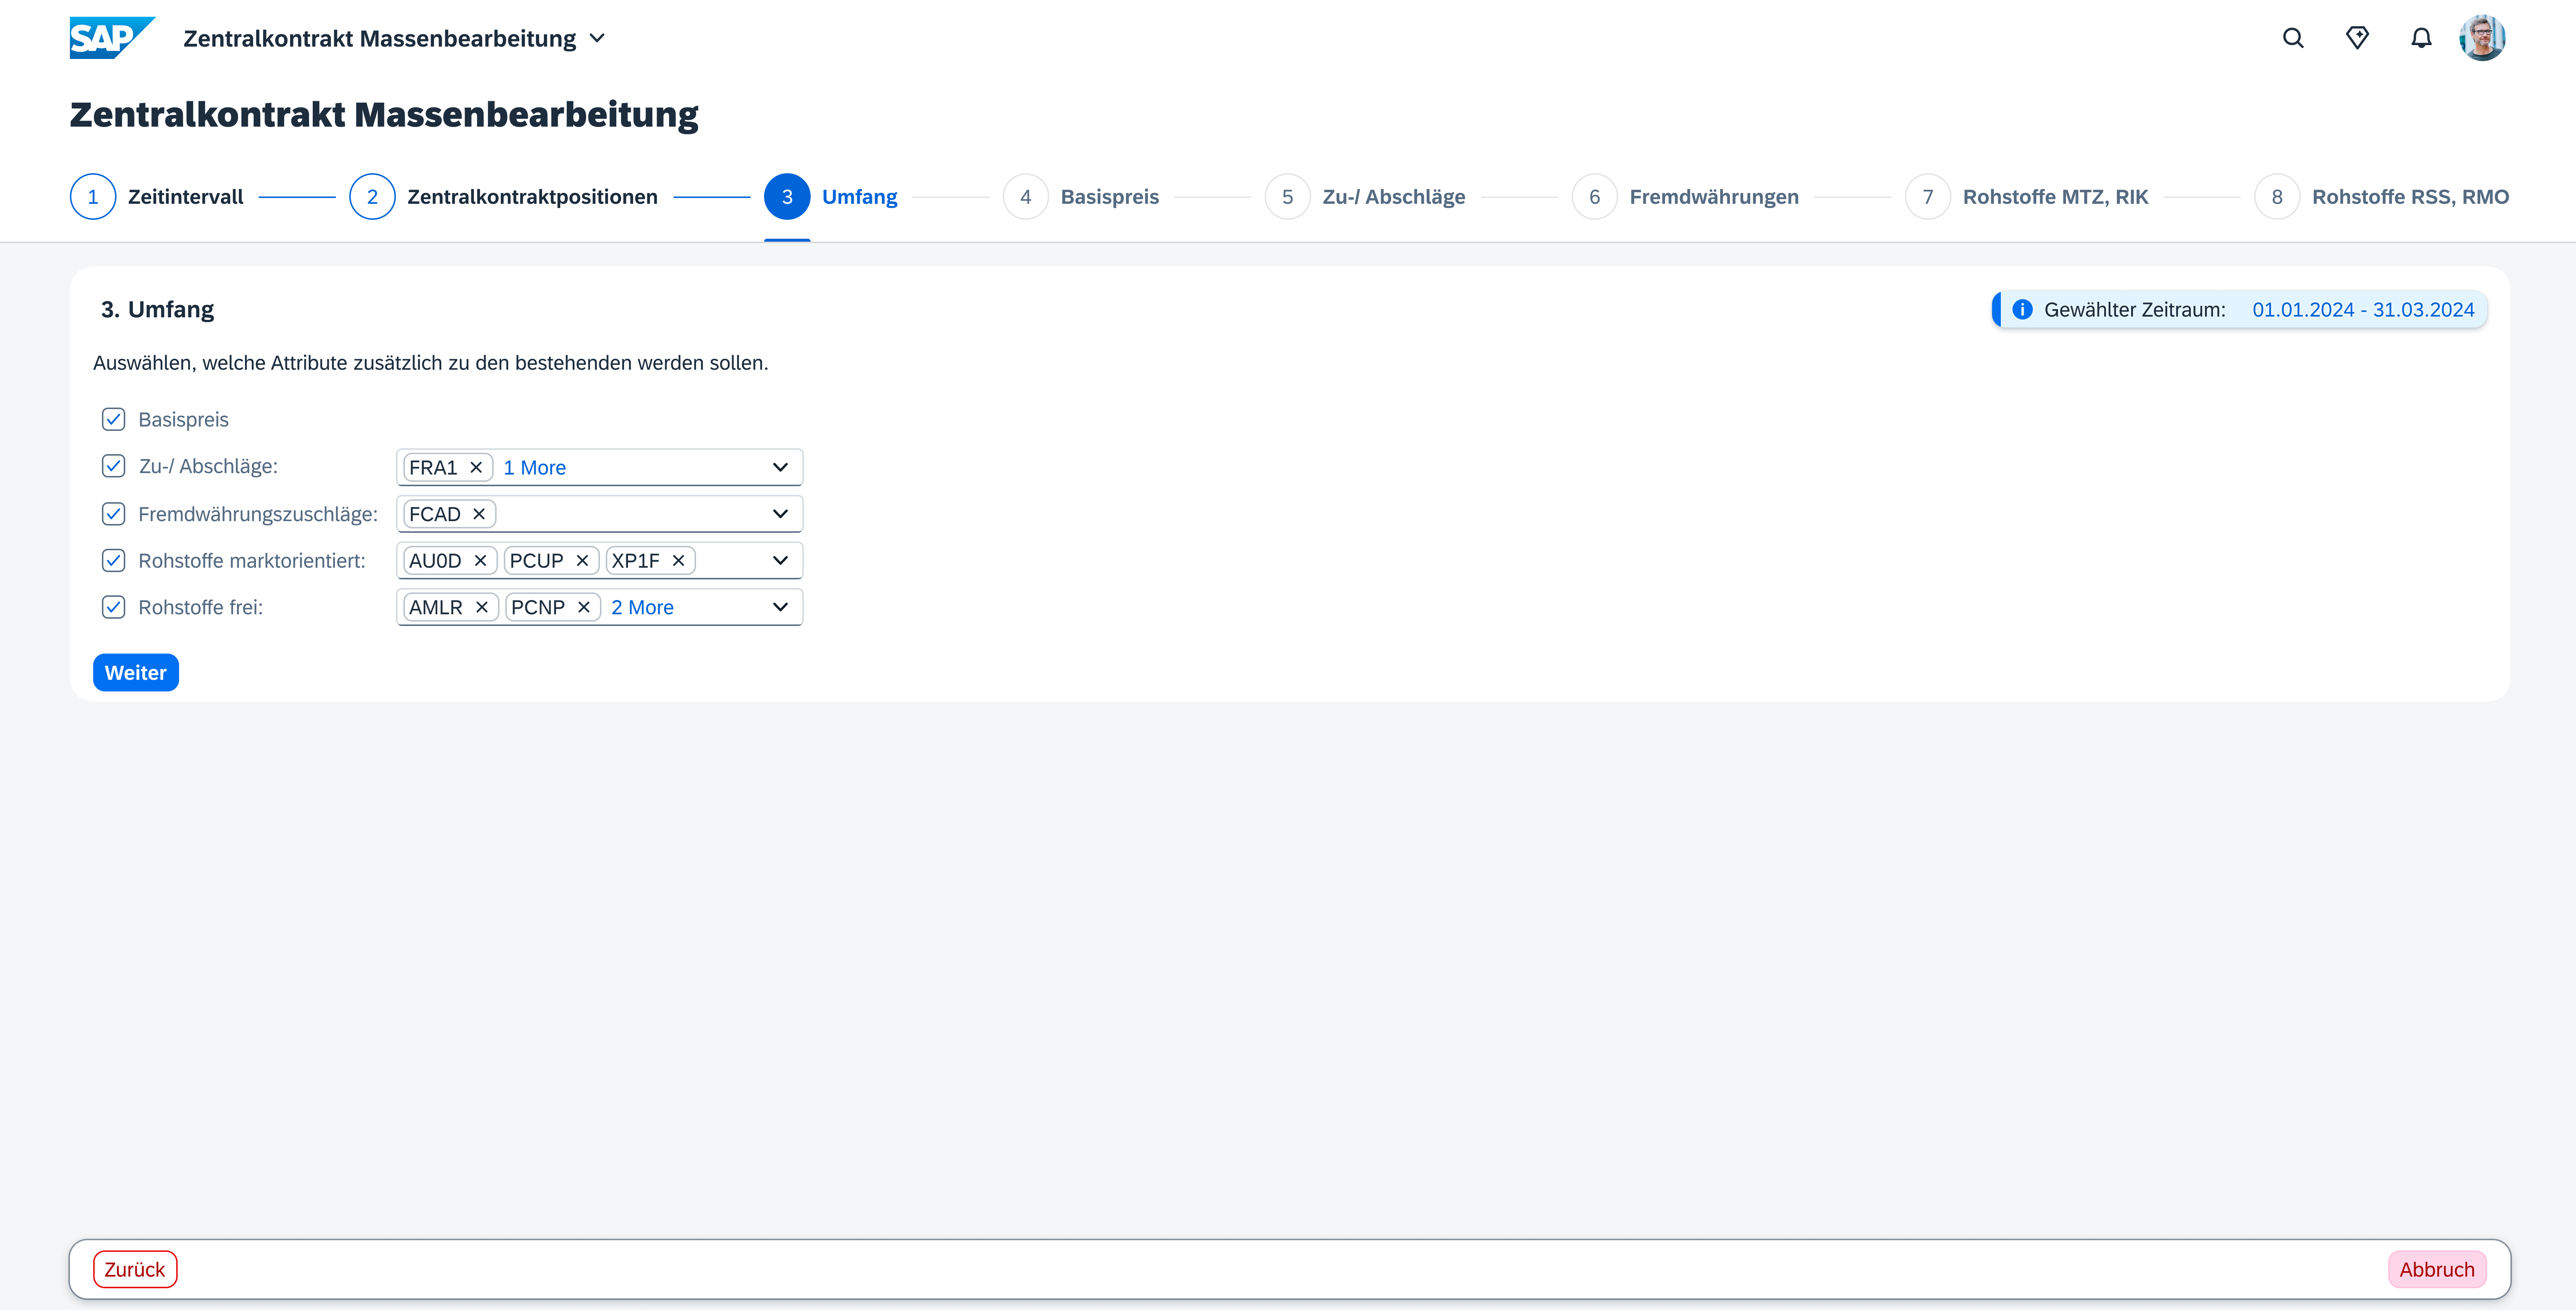
\includegraphics[height=7.65cm]{Bilder/Praxisteil-KL-Schritt-3.png}
    \caption[Kundenentwicklung, Massenbearbeitung Central Contracts, Auswahl der zu bearbeitenden Kategorien]{Kundenentwicklung, Massenbearbeitung Central Contracts, Auswahl der zu bearbeitenden Kategorien. Eigene Darstellung}
    \label{fig:PraxisKLSchritt3}
\end{figure}

Der letzte Schritt der Vorauswahl wird in Abbildung \ref{fig:PraxisKLSchritt3} dargestellt. Hier kann der Facheinkäufer durch selektieren der Checkboxen auswählen, welche der fünf Kategorien der Zentralkontrakte er bearbeiten möchte. Sollte eine Kategorie nicht selektiert sein, wird der zugehörige Prozessschritt in der App ausgeblendet. In die Inputfelder neben den Kategorien kann der Endanwender einzelne Rohstoffe oder Konditionen, wie \zB Alluminium oder einen Verpackungszuschlag mittels deren ID eingeben. Durch diese Funktionalität können neue Konditionen oder Rohstoffe hinzugefügt werden, die in den Verträgen akutell nicht vorhanden sind. Letztere werden den Tabellen im nächsten Schritt mit leeren Einträgen hinzugefügt. Alle im aktuellen Zeitintervall bestehenden Konditionen/ Rohstoffe werden, unabhängig von der Auswahl des Facheinkäufers ohnehin in den nächsten Schritten angezeigt. 

\subsubsection{Bearbeitung des Basispreises}

\begin{figure}[H]
    \centering
    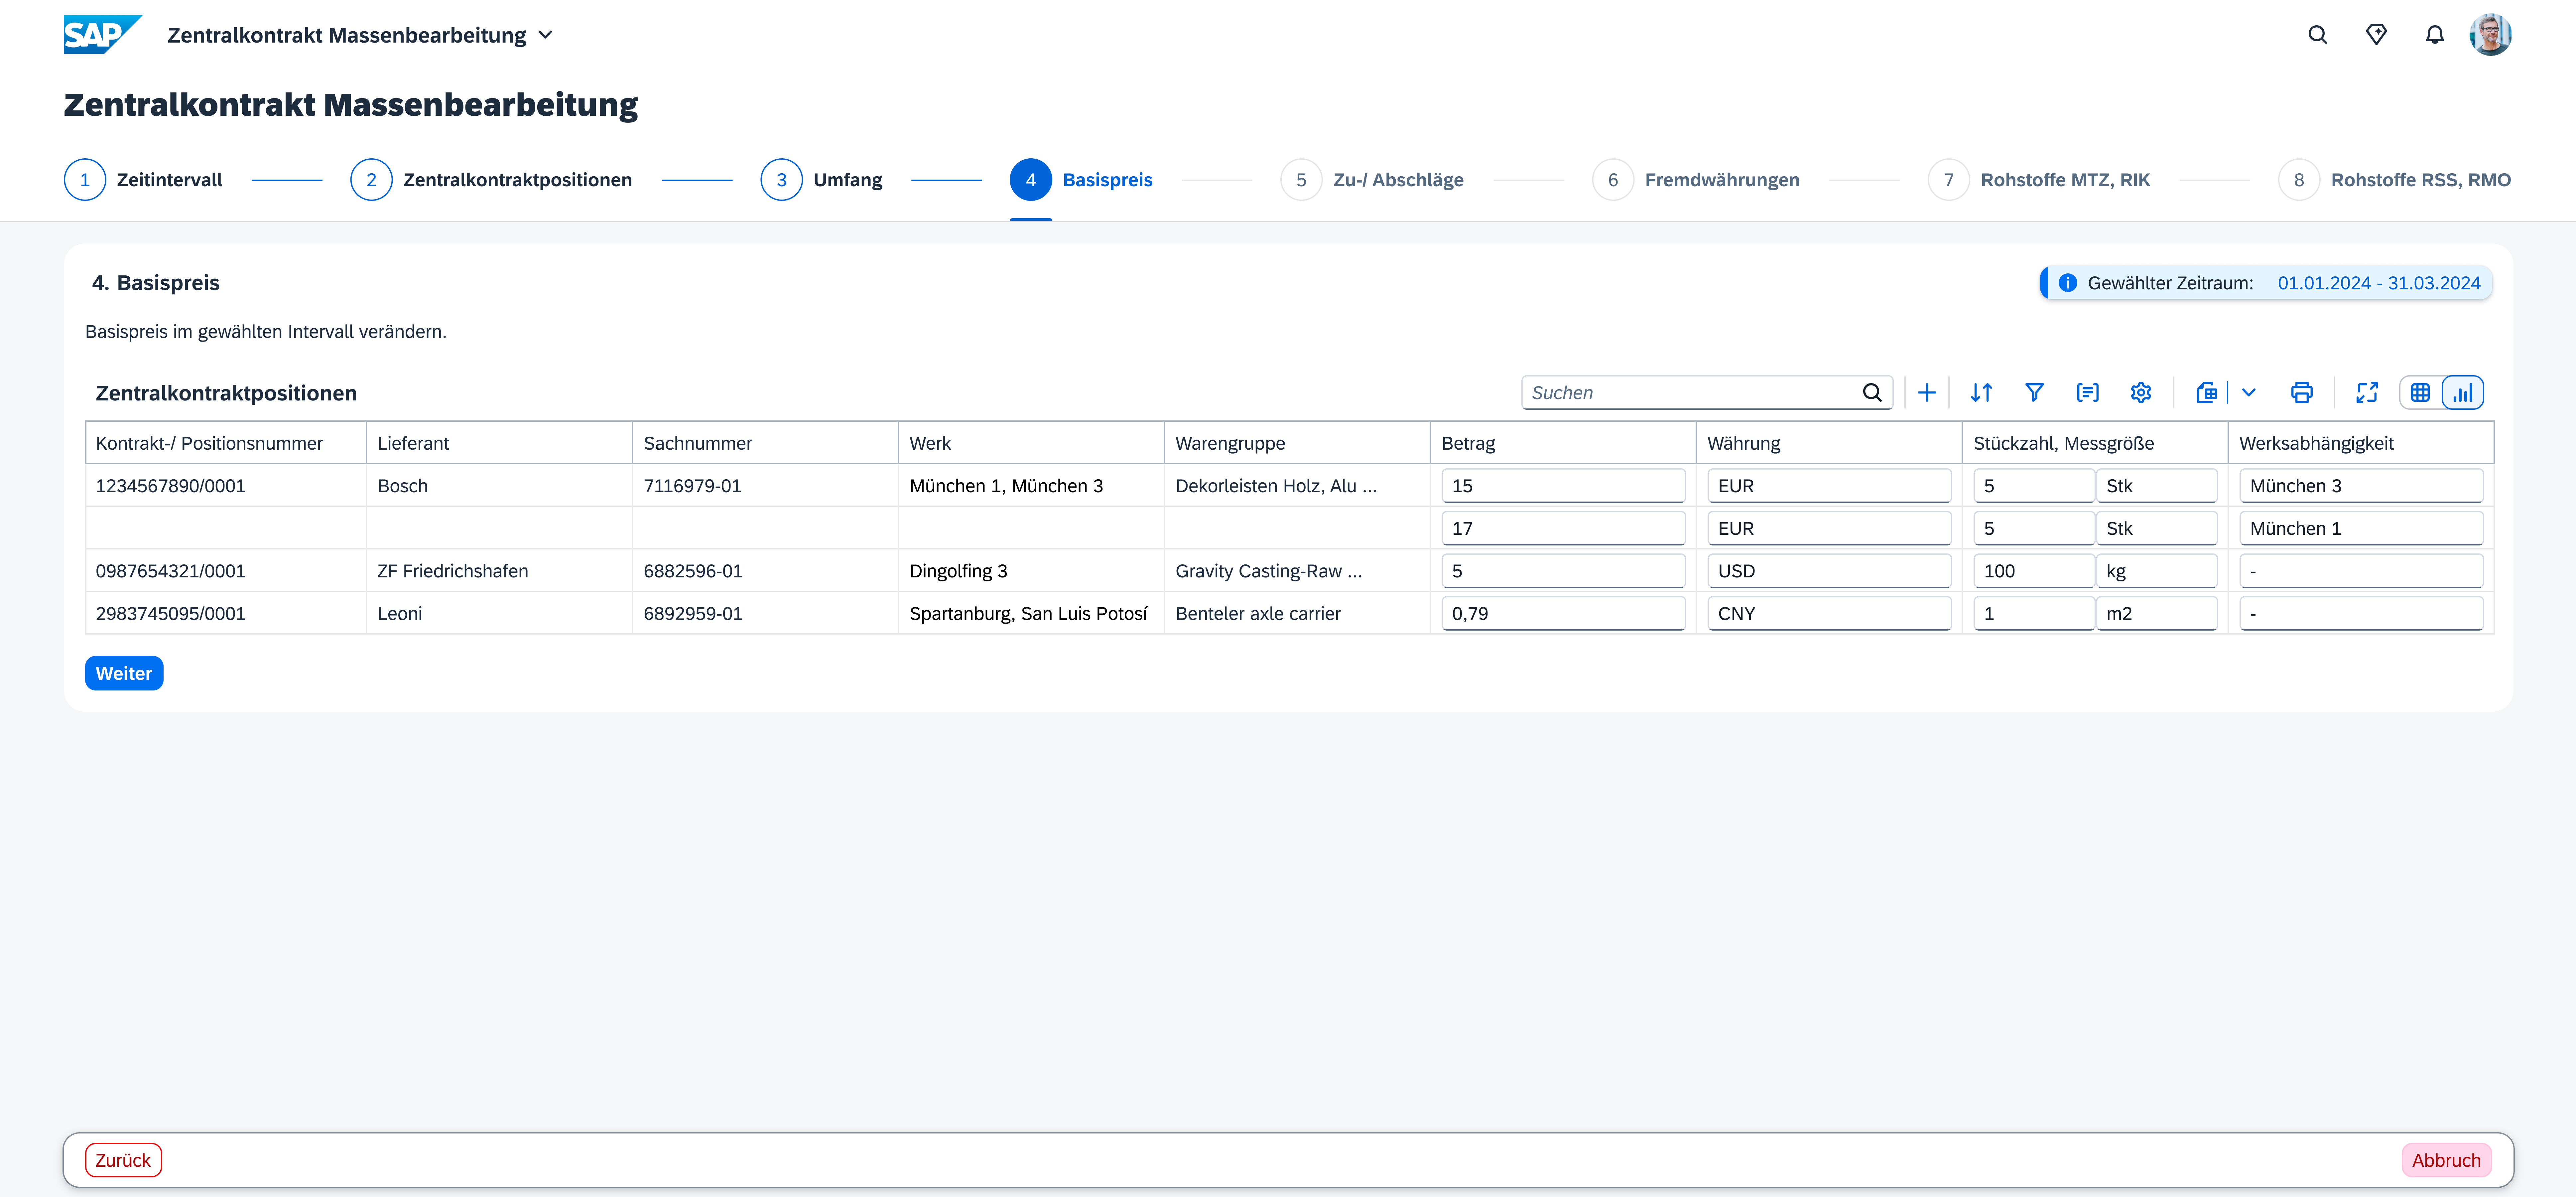
\includegraphics[height=6.99cm]{Bilder/Praxisteil-KL-Schritt-4.png}
    \caption[Kundenentwicklung, Massenbearbeitung Central Contracts, Bearbeitung des Basispreises]{Kundenentwicklung, Massenbearbeitung Central Contracts, Bearbeitung des Basispreises. Eigene Darstellung}
    \label{fig:PraxisKLSchritt4}
\end{figure}

In Abbildung \ref{fig:PraxisKLSchritt4} beginnt mit dem vierten Prozessschritt die Bearbeitungsphase mit dem Basispreis. Die Felder zur Identifikation der einzelnen Kontrakte wurden aus Übersichtlichkeitsgründen reduziert. Die jeweiligen Eingabefelder sind mit den im ausgewählten Zeitintervall gültigen Werten vorbefüllt. Sollten im gewählten Zeitintervall keine Werte vorhanden sein wären diese Felder leer. Wenn das gewählte Zeitintervall mehrere Instanzen des Basispreises mit verschiedenen Werten enthält, wird der Wert, der zu Beginn des gewählten Zeitraums gültig war, in das Feld eingetragen. Diese Logik gilt für alle weiteren anzupassenden Kategorien gleicherma\ss en. Sollte ein Vertrag werksabhängige Basispreise für verschiedene Lokationen haben, werden diese in der Tabelle in mehreren Zeilen untereinander aufgelistet. Zudem wird durch Eingaberegeln sichergestellt, dass entweder nur ein werksunabhängiger Basispreis existiert oder mehrere ausschlie\ss lich werksabhängige Basispreise. Die PME (Stückzahl, Messgrö\ss e) ist in zwei Eingabefelder aufgeteilt, um die Dateneingabe und -verarbeitung zu erleichtern. Falls ein Anwender die Dateneingabe in Excel präferiert, ist dies durch den Excel Up- und Download möglich. Es kann im Gegensatz zur Standardfunktionalität jedoch keine Datei für alle Kategorien heruntergeladen werden, sondern lediglich eine Datei pro Kategorie, die schematisch der in Abbildung \ref{fig:PraxisKLSchritt4} dargestellten Tabelle entspricht. Diese kann mit den aktuellen Werten befüllt heruntergeladen, angepasst und wieder hochgeladen werden. Somit kann die Fehlerbehandlung immernoch durch die App erfolgen, da eventuelle Falscheingabe farblich und mit einer Benachrichtigung hervorgehoben werden.

\subsubsection{Bearbeitung der Zu- und Abschläge}

\begin{figure}[H]
    \centering
    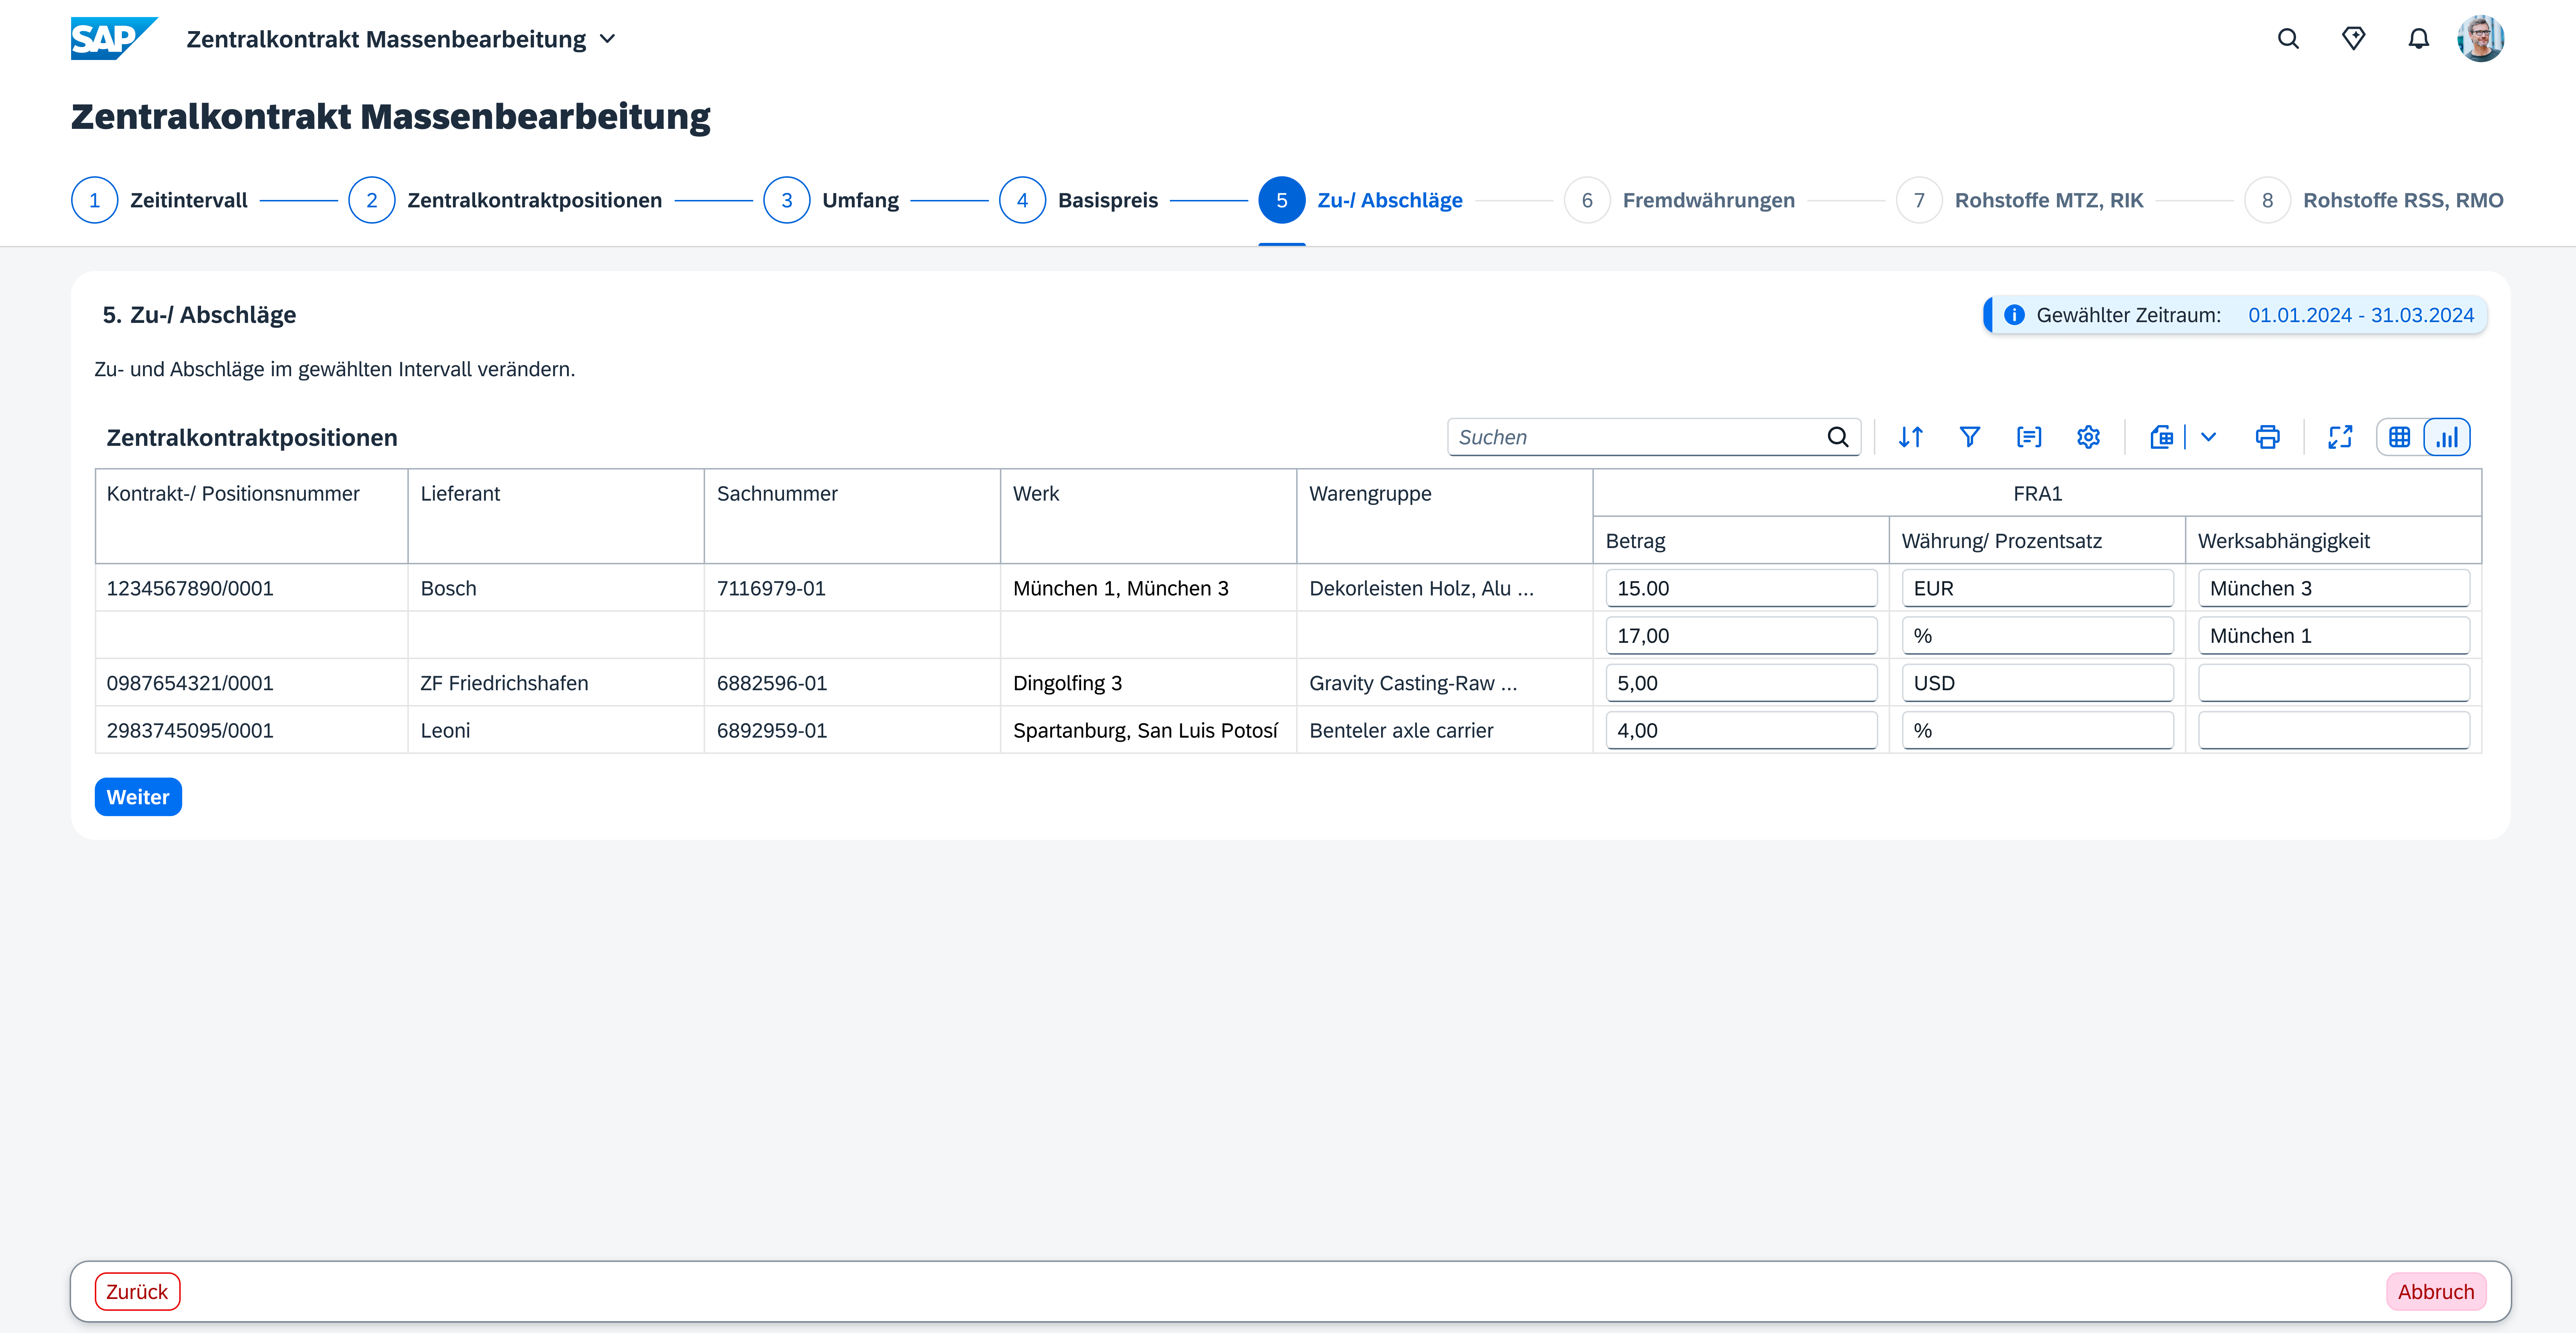
\includegraphics[height=7.78cm]{Bilder/Praxisteil-KL-Schritt-5.png}
    \caption[Kundenentwicklung, Massenbearbeitung Central Contracts, Bearbeitung der Zu- und Abschläge]{Kundenentwicklung, Massenbearbeitung Central Contracts, Bearbeitung der Zu- und Abschläge. Eigene Darstellung}
    \label{fig:PraxisKLSchritt5}
\end{figure}

Nachdem der Basispreis bearbeitet wurde, ist der nächste Schritt in Abbildung \ref{fig:PraxisKLSchritt5} die Bearbeitung der Zu- und Abschläge. Diese werden in der Tabelle in Spalten dargestellt, die sich in die je relevanten Felder unterteilen. Im konkreten Beispiel handelt es sich um einen Frachtzuschlag, der je nach Vertrag und Werksabhängigkeit andere Werte annehmen kann.\footnote{Aus Darstellungsgründen wurde auf die Darstellung mehrerer Zuschläge verzichtet. Diese würden analog zu ''FRA1'' rechts an die Tabelle ''angehängt'' werden. Selbiges gilt für die nächsten Kateogrien, die im Folgenden vorgestellt werden.} Im Unterschied zum Basispreis existiert das Feld PME nicht, da sich diese Konditionsart immer auf den gesamten Basispreis und nicht auf eine bestimmte Mengeneinheit bezieht. Des Weiteren kann ein Zu- bzw. Abschlag auch in Prozent auf den Basispreis angegeben werden. Das Feld ''Betrag'' wird automatisch in Abhängigkeit davon, ob ein Währungscode oder ''\%'' angegeben wurde interpretiert, sodass keine Umrechnung in verschiedene Dezimalstellen notwendig ist. Beispielsweise kann der Einkäufer einen Frachtzuschlag von 0,5\% als ''0,5'' eingeben und muss diesen nicht als ''0,005'' eingeben. In allen editierbaren Kategorien - au\ss er des Basispreises - können \zB einzelne Rohstoffe oder Zu-/ Abschläge für einen Kontrakt gelöscht werden. Dies wird durch das Löschen aller Werte in den entsprechenden Feldern eines Zuschlags für einen bestimmten Vertrag durchgeführt. Der Basispreis hingegen kann für ein gültiges Zeitintervall nicht gelöscht, sondern nur überschrieben werden, da sonst Lücken im Preisverlauf entstehen würden. 

\subsubsection{Bearbeitung der Fremdwährungen}

\begin{figure}[H]
    \centering
    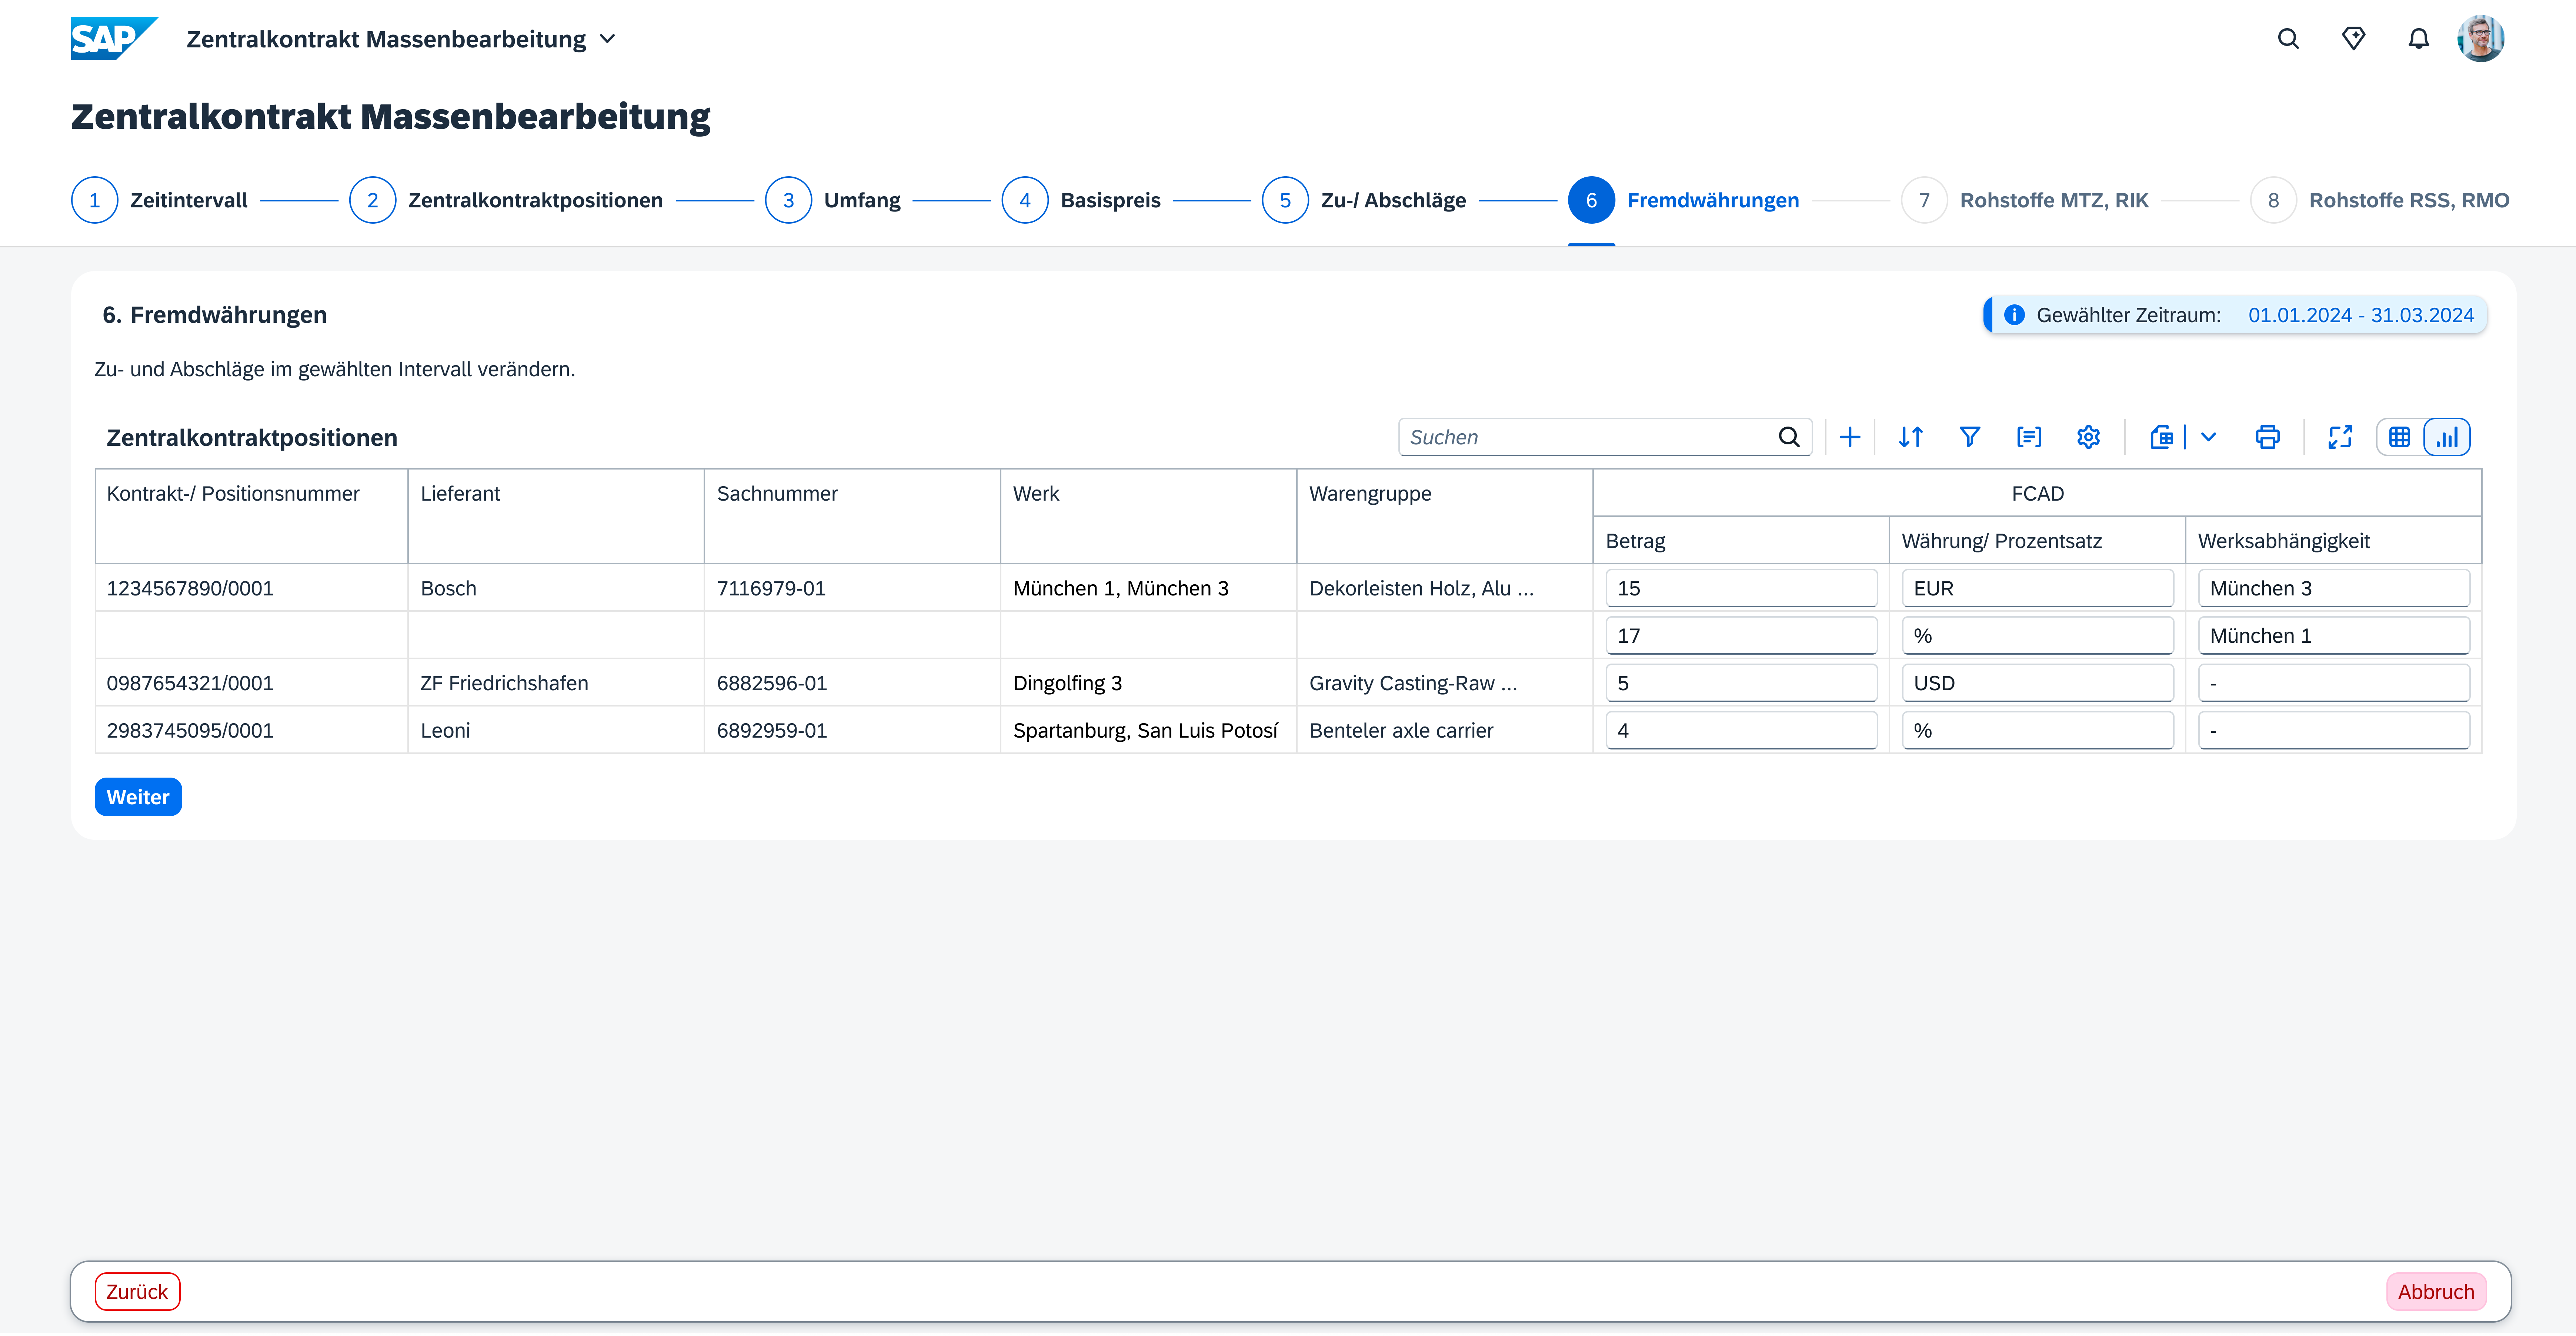
\includegraphics[height=7.78cm]{Bilder/Praxisteil-KL-Schritt-6.png}
    \caption[Kundenentwicklung, Massenbearbeitung Central Contracts, Bearbeitung der Fremdwährungen]{Kundenentwicklung, Massenbearbeitung Central Contracts, Bearbeitung der Fremdwährungen. Eigene Darstellung}
    \label{fig:PraxisKLSchritt6}
\end{figure}

Die nächste Konditionsart sind Fremdwährungen, die in Abbildung \ref{fig:PraxisKLSchritt6} dargestellt sind. Diese sind im Bezug auf die benötigten Felder analog zu den Zu- und Abschlägen aufgebaut. Der Unterschied besteht lediglich darin, dass der Zweck spezialisiert ist, um internationale Währungsdifferenzen zu berücksichtigen.

\subsubsection{Bearbeitung der marktorientierten Rohstoffe}

\begin{figure}[H]
    \centering
    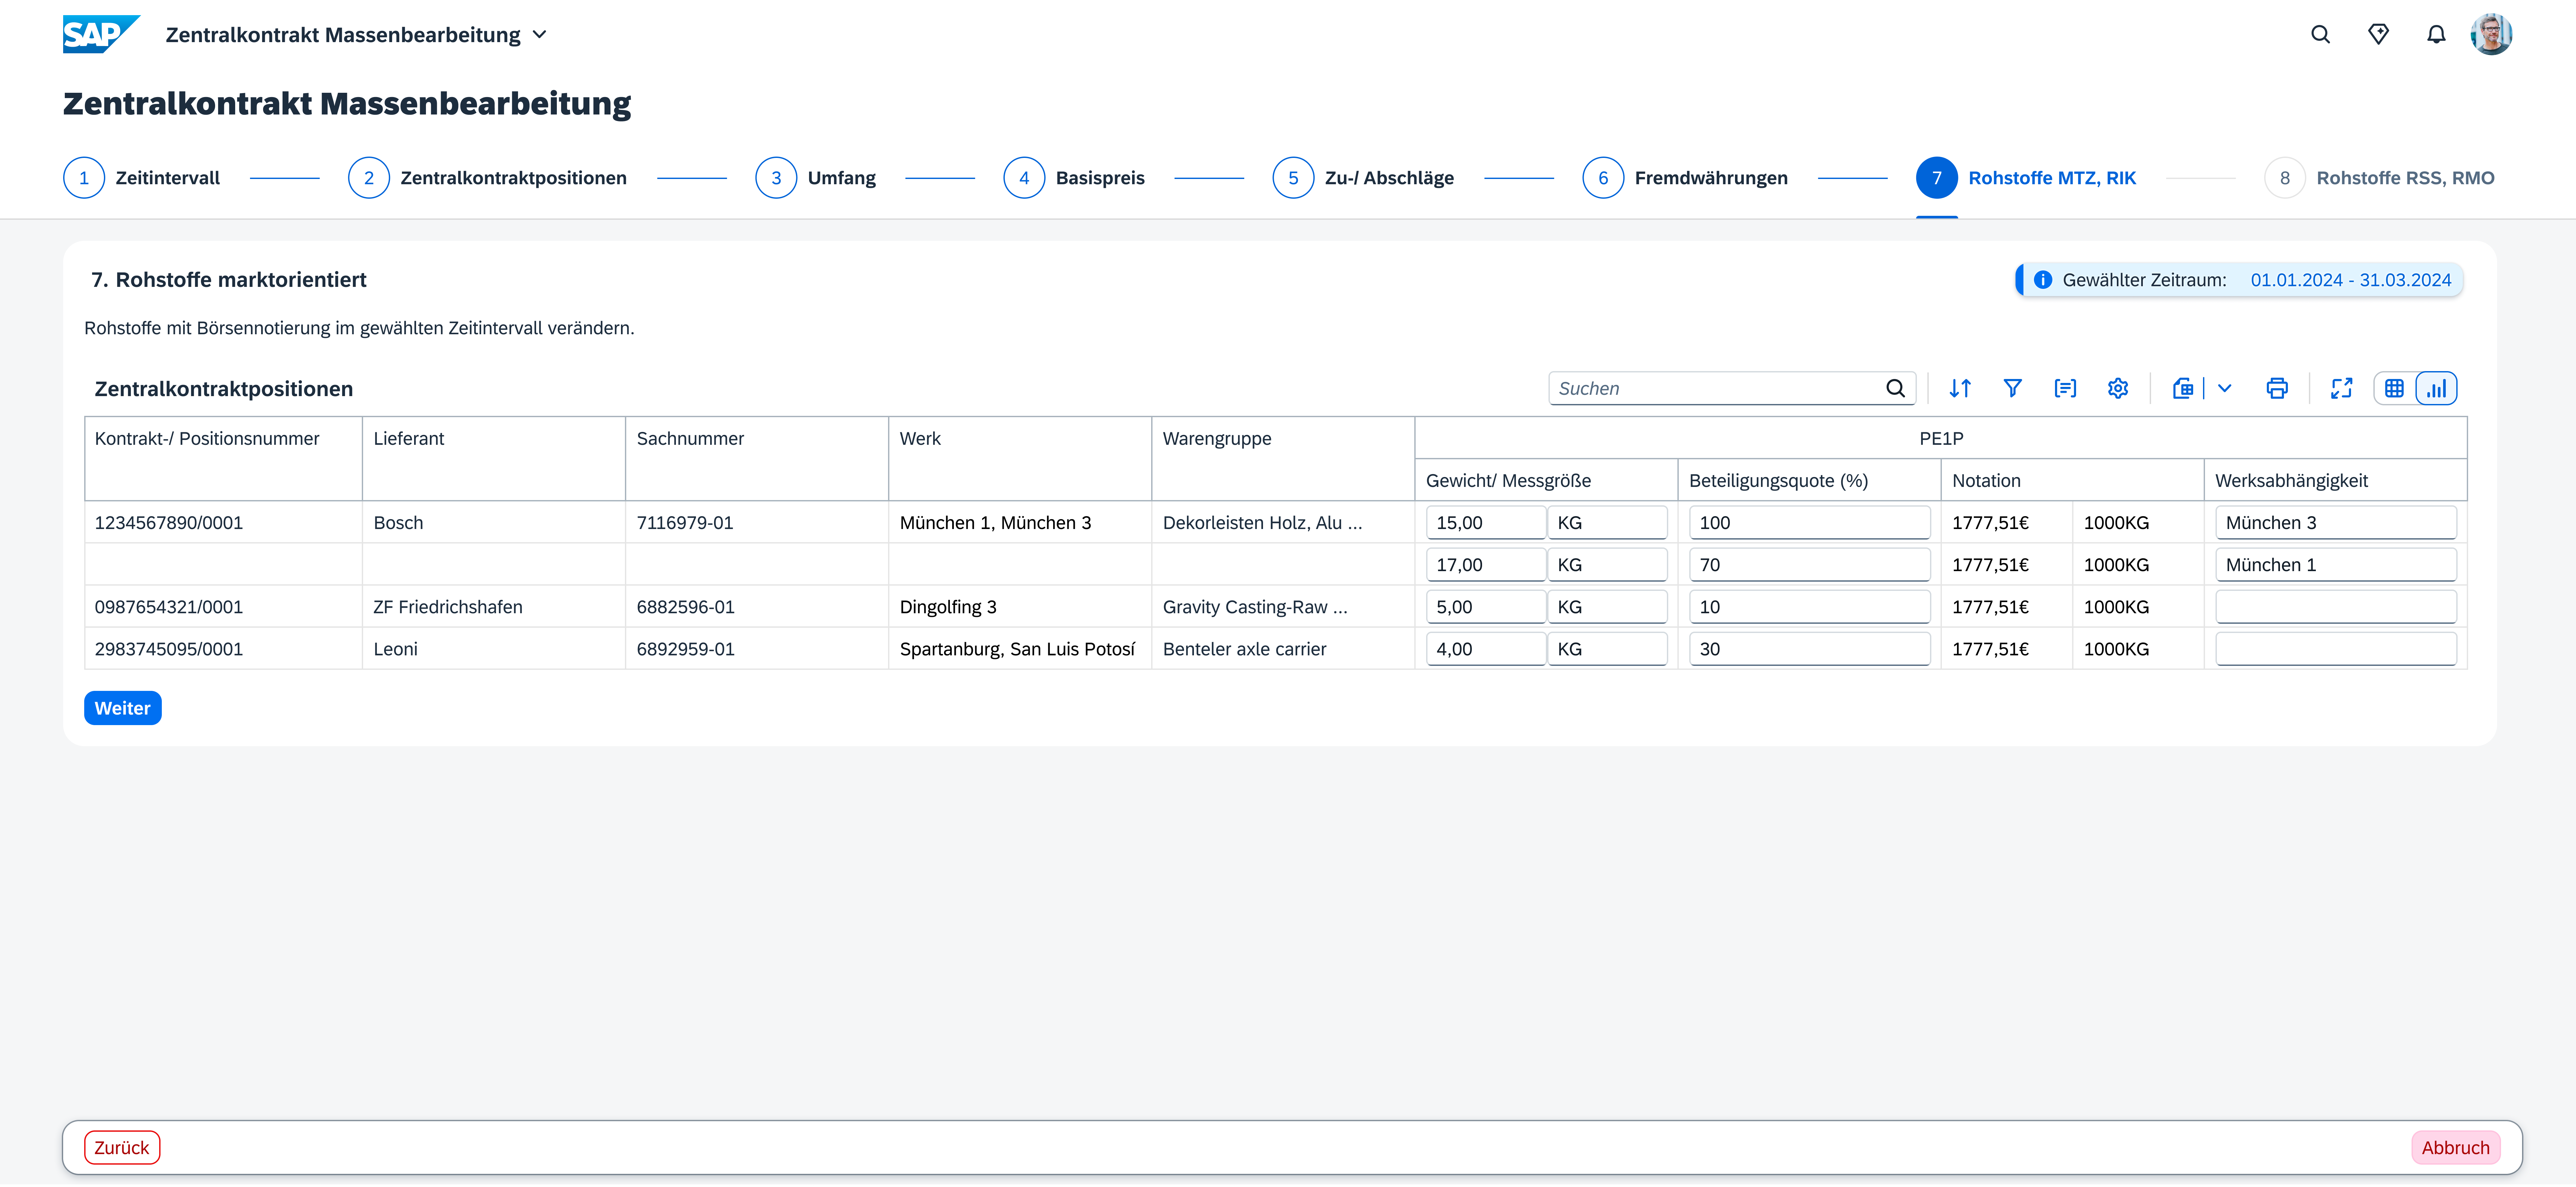
\includegraphics[height=6.91cm]{Bilder/Praxisteil-KL-Schritt-7.png}
    \caption[Kundenentwicklung, Massenbearbeitung Central Contracts, Bearbeitung der marktorientierten Rohstoffe]{Kundenentwicklung, Massenbearbeitung Central Contracts, Bearbeitung der marktorientierten Rohstoffe. Eigene Darstellung}
    \label{fig:PraxisKLSchritt7}
\end{figure}

Die letzten beiden Kategorien, die der Endanwender bearbeiten kann, sind Rohstoffe. In Abbildung \ref{fig:PraxisKLSchritt7} ist die Maske für marktorientierte Rohstoffe dargestellt. Da die Notationen der RMO vom organisierten Markt vorgegeben werden, sind diese als normale Textfelder angelegt und somit nicht durch den Anwender veränderbar. Letztere ist zudem in zwei Felder aufgegliedert, da der Preis sich immer auf eine bestimmte Menge des Rohstoffs bezieht. Um die gesamte preisliche Auswirkung auf den Basispreis zu erfassen, ist zudem noch die Menge des Rohstoffs, die für ein Bauteil benötigt wird, zu erfassen. Abhängig von der Art des Bauteils kann diese Menge in verschiedenen Einheiten angegeben werden. Beispielsweise wäre in einem Karrosseriebauteil wesentlich mehr Alluminium enthalten, als in einem Computerchip Silizium enthalten ist. Die eingegebenen Daten werden noch mit der Beteiligungsquote multipliziert, um den tatsächlichen Rohstoffpreis in einem Bauteil zu berechnen. Sie gibt an, zu welchem Anteil BMW sich an dem Rohstoff-Preisbestandteil beteiligt und ist somit wichtig, um Preisschwankungen abzufedern.

\subsubsection{Bearbeitung der Rohstoffe mit freier Notierung}

\begin{figure}[H]
    \centering
    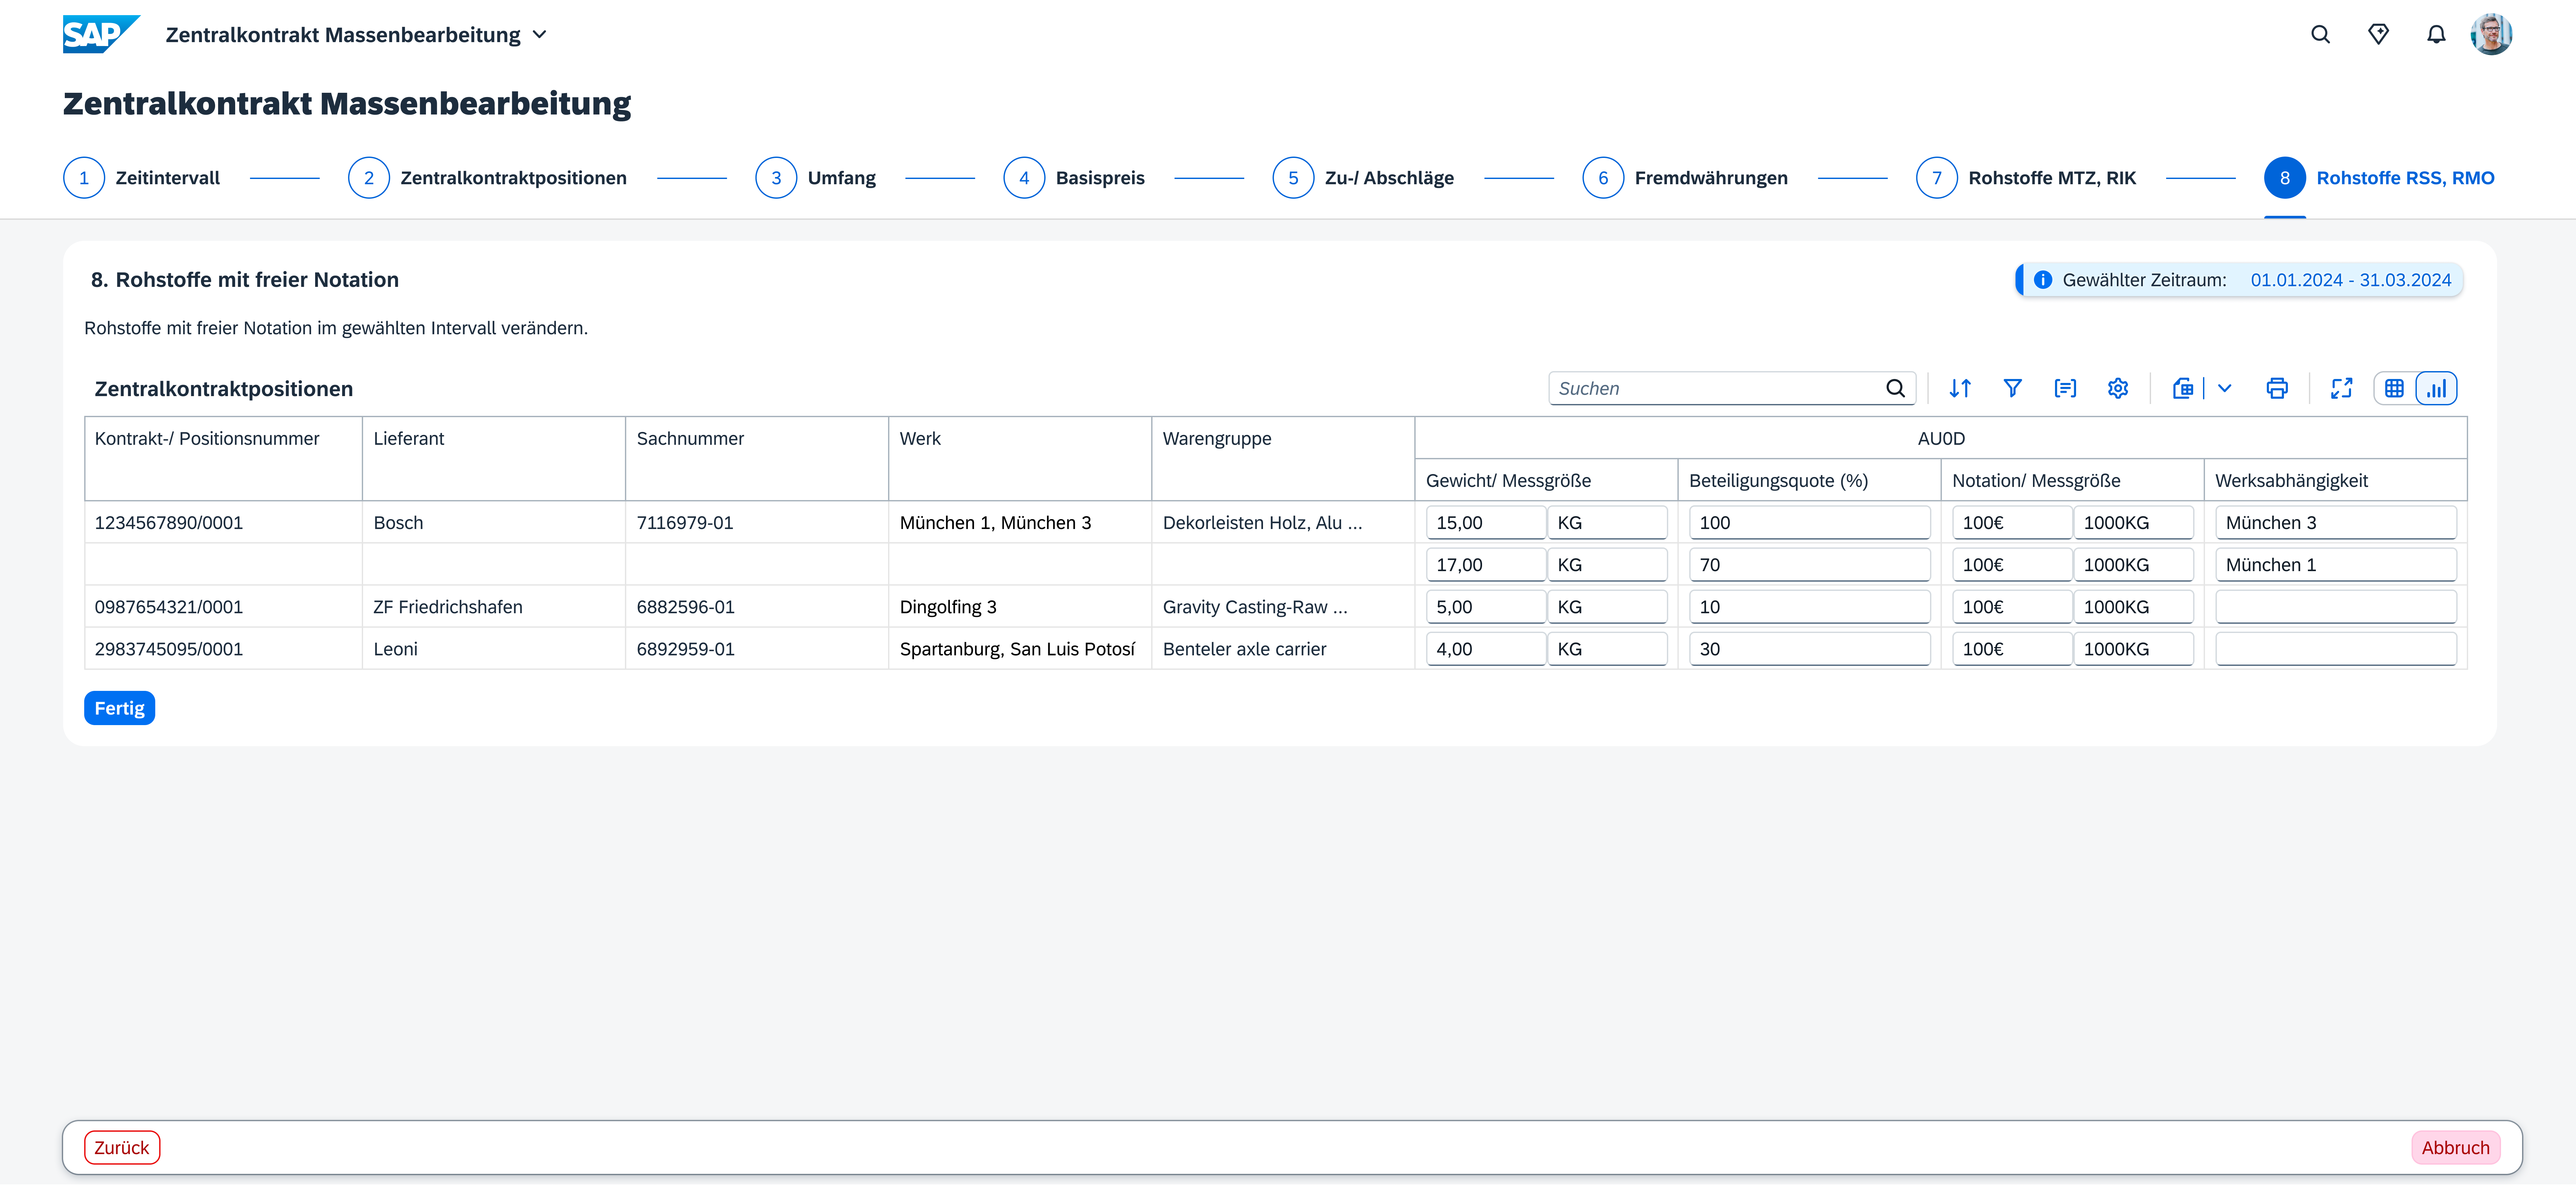
\includegraphics[height=6.91cm]{Bilder/Praxisteil-KL-Schritt-8.png}
    \caption[Kundenentwicklung, Massenbearbeitung Central Contracts, Bearbeitung der Rohstoffe mit freier Notierung]{Kundenentwicklung, Massenbearbeitung Central Contracts, Bearbeitung der Rohstoffe mit freier Notierung. Eigene Darstellung}
    \label{fig:PraxisKLSchritt8}
\end{figure}

Der letzte Prozessschritt ist die Bearbeitung der Rohstoffe mit freier Notierung. Diese sind in Abbildung \ref{fig:PraxisKLSchritt8} dargestellt und ebenfalls ähnlich zu den RMO aufgebaut. Der Unterschied besteht darin, dass die Preise nicht vorgegeben werden, sondern vom Facheinkäufer selbst gepflegt werden können. Aus diesem Grund ist die Notation als Inputfeld angelegt.

Nachdem der Einkäufer alle Änderungen bestätigt hat, wird im Hintergrund eine Schnittstelle der Lösung Contract Price Renegotiation aufgerufen. Diese übernimmt einerseits die Anpassung der Preisgültigkeiten (automatische Verkürzung und Verlängerung der Basispreis-Intervalle, quartalsweise Trennung von Rohstoffgültigkeiten) und andererseits die Übernahme der Daten ins System. Mit diesem Schritt ist der Prozess abgeschlossen.

\section{Evaluation der verschiedenen Lösungsansätze}

-> Nutzwertanalyse (siehe 1.4)